\documentclass[12pt]{article}
\usepackage[utf8]{inputenc}
\usepackage[dvipsnames]{xcolor}
%\usepackage[usenames]{color}
\usepackage{graphicx}
\usepackage{subfigure}
\usepackage[natbibapa]{apacite}
\bibliographystyle{apacite}
\graphicspath{ {images/} }
\usepackage{vmargin}
\usepackage{amsmath}
\usepackage{circuitikz}
\usepackage{tikz}
\usepackage{tocloft}
\usetikzlibrary{calc}
\usetikzlibrary{arrows}
\usepackage{pgfplots}
\usepackage{units}
\usetikzlibrary{patterns}
\usepackage{setspace}
\usepackage{multicol}
\usepackage{multirow}
\usepackage{colortbl}
\usepackage{array}
\usepackage{booktabs}
\usepackage{caption}
\usepackage{amssymb}
\usepackage{amsfonts}
\usepackage{amsthm}
\usepackage{amsmath,yhmath}
\usepackage{geometry}
%\usepackage{subcaption}
\usepackage{graphicx}
\usepackage[export]{adjustbox}
\usepackage[framemethod=tikz]{mdframed}
\usepackage{lipsum}
\usepackage{tcolorbox}
\usepackage{tocloft}
%\usepackage[colorlinks,citecolor=red]{hyperref}
%\usepackage{}
%\newtcolorbox{mybox2}{colback=red!5!white,colframe=red!75!black,width=0.85\textwidth}
\newtcolorbox{mybox2}[1]{colback=gray!5!white,colframe=cyan!75!black,fonttitle=\bfseries,title=#1}

\newtcolorbox{mybox3}[1]{colback=gray!5!white,colframe=Maroon!75!black,fonttitle=\bfseries,title=#1}

\newtcolorbox{mybox4}[1]{colback=gray!5!white,colframe=LimeGreen!75!black,fonttitle=\bfseries,title=#1}


\newcommand{\listequationsname}{\Large Lista de ecuaciones}
\newlistof{myequations}{equ}{\listequationsname}
\newcommand{\myequations}[1]{%
\addcontentsline{equ}{myequations}{Ecuación\hspace{0.3em}\protect\numberline{\theequation}#1}\par}
\setlength{\cftmyequationsnumwidth}{1.75em}
\setlength{\cftmyequationsindent}{1.5em}
\addtocontents{equ}{~\hfill\textbf{Página}\par}


\definecolor{mycolor}{rgb}{0.122, 0.435, 0.698}
%\captionsetup[table]{name=Tabla}
%\usepackage{bigstrut}
\setpapersize{A4}
\setmargins{2.5cm}       % margen izquierdo
{1.5cm}                        % margen superior
{16.5cm}                      % anchura del texto
{23.42cm}                    % altura del texto
{10pt}                           % altura de los encabezados
{1cm}                           % espacio entre el texto y los encabezados
{0pt}                             % altura del pie de página
{2cm}                           % espacio entre el texto y el pie de página
\usepackage{diagbox}
\usepackage{slashbox}
\newtheorem{defi}{Inciso}[subsection]
\renewcommand{\listfigurename}{Lista de Figuras}
\renewcommand{\listtablename}{Lista de Tablas}
\renewcommand{\baselinestretch}{1.5}
\renewcommand{\abstractname}{Resumen}
\renewcommand{\figurename}{Figura}
\renewcommand{\contentsname}{\underline{Contenido}}
\renewcommand{\tablename}{Tabla}

\renewcommand{\cftfigfont}{Figura }
\renewcommand{\cfttabfont}{Tabla }
\addtocontents{toc}{~\hfill\textbf{Página}\par}
\addtocontents{lot}{~\hfill\textbf{Página}\par}
\addtocontents{lof}{~\hfill\textbf{Página}\par}
\providecommand{\keywords}[1]
{
  \textbf{\text{Palabras clave: }} #1
}

\title{\textbf{MEMORIA DE CALCULO ESTRUCTURAL}}
\author{VIVIENDA MULTIFAMILIAR}
\date{Junio 06, 2002}
\usepackage[hidelinks]{hyperref}
\begin{document}
\maketitle
\begin{figure}[h!]
    \centering
    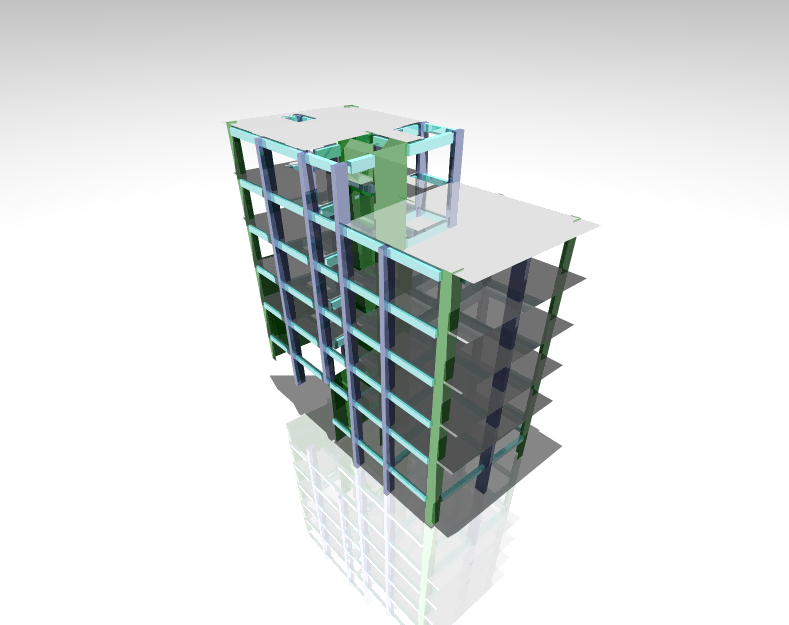
\includegraphics[scale=0.75]{IMAGENES/r2.png}
    \label{fig:my_label}
\end{figure}
\thispagestyle{empty}
\newpage
  \begin{spacing}{1.35}
    \tableofcontents
  \end{spacing}
\thispagestyle{empty}
\listoffigures
\thispagestyle{empty}
\listoftables
\thispagestyle{empty}
\listofmyequations
\newpage

\begin{abstract}
\thispagestyle{empty}
El presente documento contempla todo lo concerniente al análisis estructural de la vivienda multifamiliar para acciones gravitacionales y sísmicas según lo establecido en el reglamento nacional de edificaciones vigente. De manera preliminar se presentan los datos de la edificación como la ubicación, planta y elevación arquitectónica, resultados y recomendaciones del estudio de mecánica de suelos. Posterior a esto se realiza la estructuración y el predimensionamiento de los elementos estructurales siguiendo lo establecido en las normas y recomendaciones de especialistas en la rama. Finalmente se realiza el análisis sísmico según la norma E-030, se verifica las irregularidades y se construye el espectro de respuesta de aceleraciones que representa la demanda sísmica, se realiza el análisis modal y se determina las dimensiones finales de los elementos para dotar al edificio de suficiente rigidez lateral para cumplir la deriva máxima permisible en estructuras de concreto armado, finalmente se verifica el sistema estructural y se escala las fuerzas obtenidas con el análisis dinámico modal espectral al porcentaje mínimo respecto a la cortante basal estática para combinar las fuerzas con las acciones gravitacionales según lo establecido en la norma E-060. La estructura resultante consiste en un sistema estructural de muros en la dirección X y de pórticos en la dirección Y, y derivas máximas de aproximadamente 0,0035 en la dirección X y 0.006 en Y.
\vfill
\begin{flushleft}
\keywords{Vivienda multifamiliar, Análisis sísmico, E-030, E-060.}
\end{flushleft}

\end{abstract}
\newpage
\section{Datos de la edificación}

% Table generated by Excel2LaTeX from sheet 'Hoja1'
\begin{table}[htbp]
  \centering
  %\caption{Add caption}
    \begin{tabular}{lrl}
    PROYECTO  & :     & CONSTRUCCION VIVIENDA MULTIFAMILIAR \\
          &       &  \\ 
    UBICACIÓN & :     & AV. CHINCHAYSUYO – AYUDA MUTUA Lt 03 Mz 03 \\
          &       &  \\
    DISTRITO & :     & CUSCO \\
          &       &  \\
    PROVINCIA & :     & CUSCO \\
          &       &  \\
    DEPARTAMENTO & :     & CUSCO \\
    \end{tabular}%
  \label{tab:addlabel}%
\end{table}%
\vspace{-0.8cm}

\section{Estudio de mecánica de suelos (EMS)}

\subsection{Perfil de suelo}

\begin{figure}[h!]
    \centering
    \caption{Clasificación del suelo}
    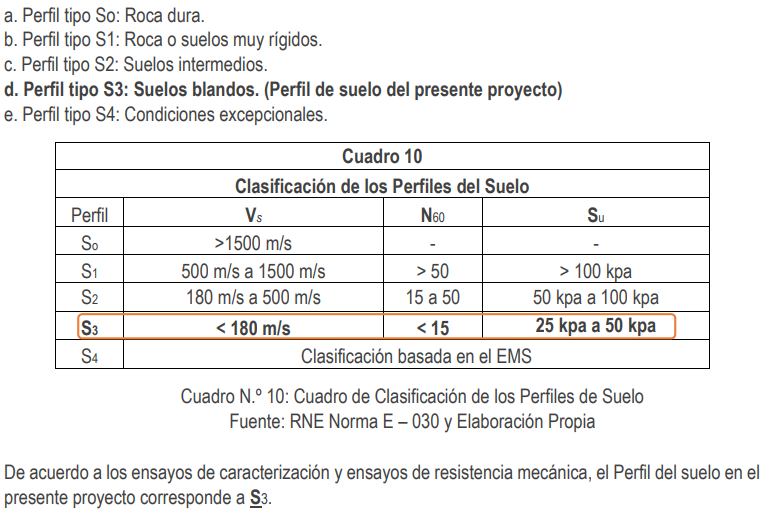
\includegraphics[scale=0.85]{IMAGENES/1.PNG}
    \caption*{\small Fuente: \it EMS}
    \label{fig:my_label}
\end{figure}

\newpage
\subsection{Profundidad de cimentación y capacidad portante}

\begin{figure}[h!]
    \centering
    \caption{Profundidad de cimentación}
    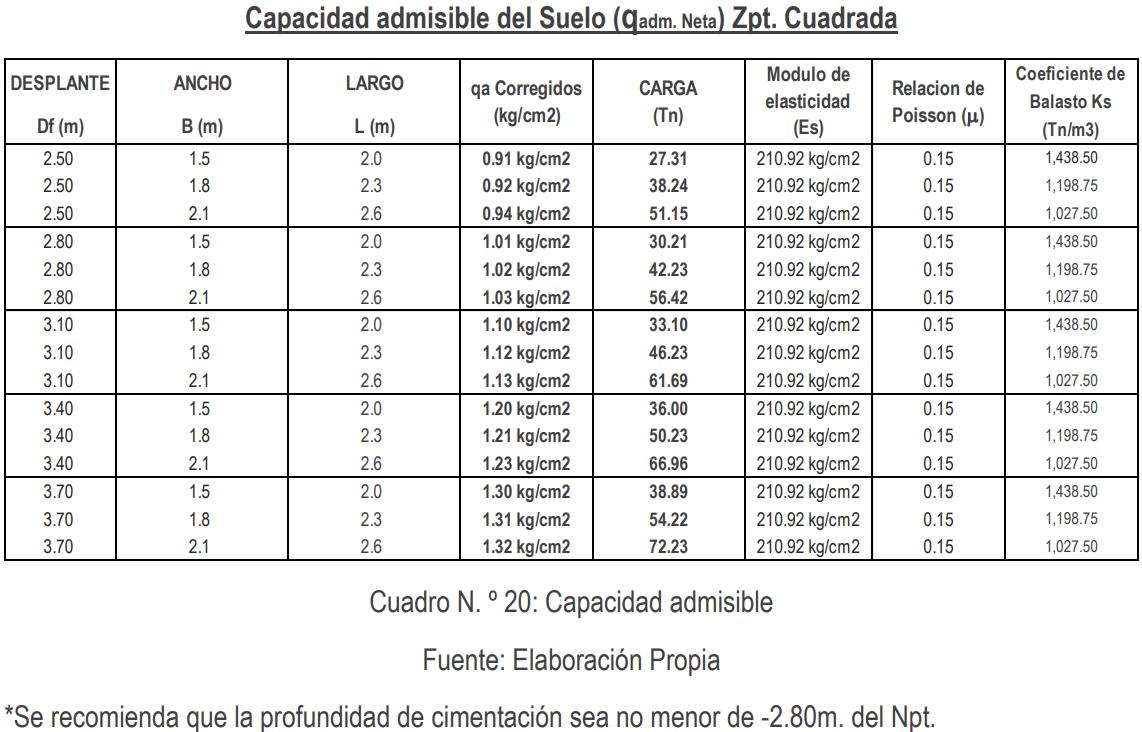
\includegraphics[scale=0.6]{IMAGENES/2.PNG}
    \caption*{\small Fuente: \it EMS}
    \label{fig:my_label}
\end{figure}

\section{Arquitectura}
Ver figuras \ref{pl} y \ref{el}.
\begin{figure}[h!]
    \centering
    \caption{Planta}
    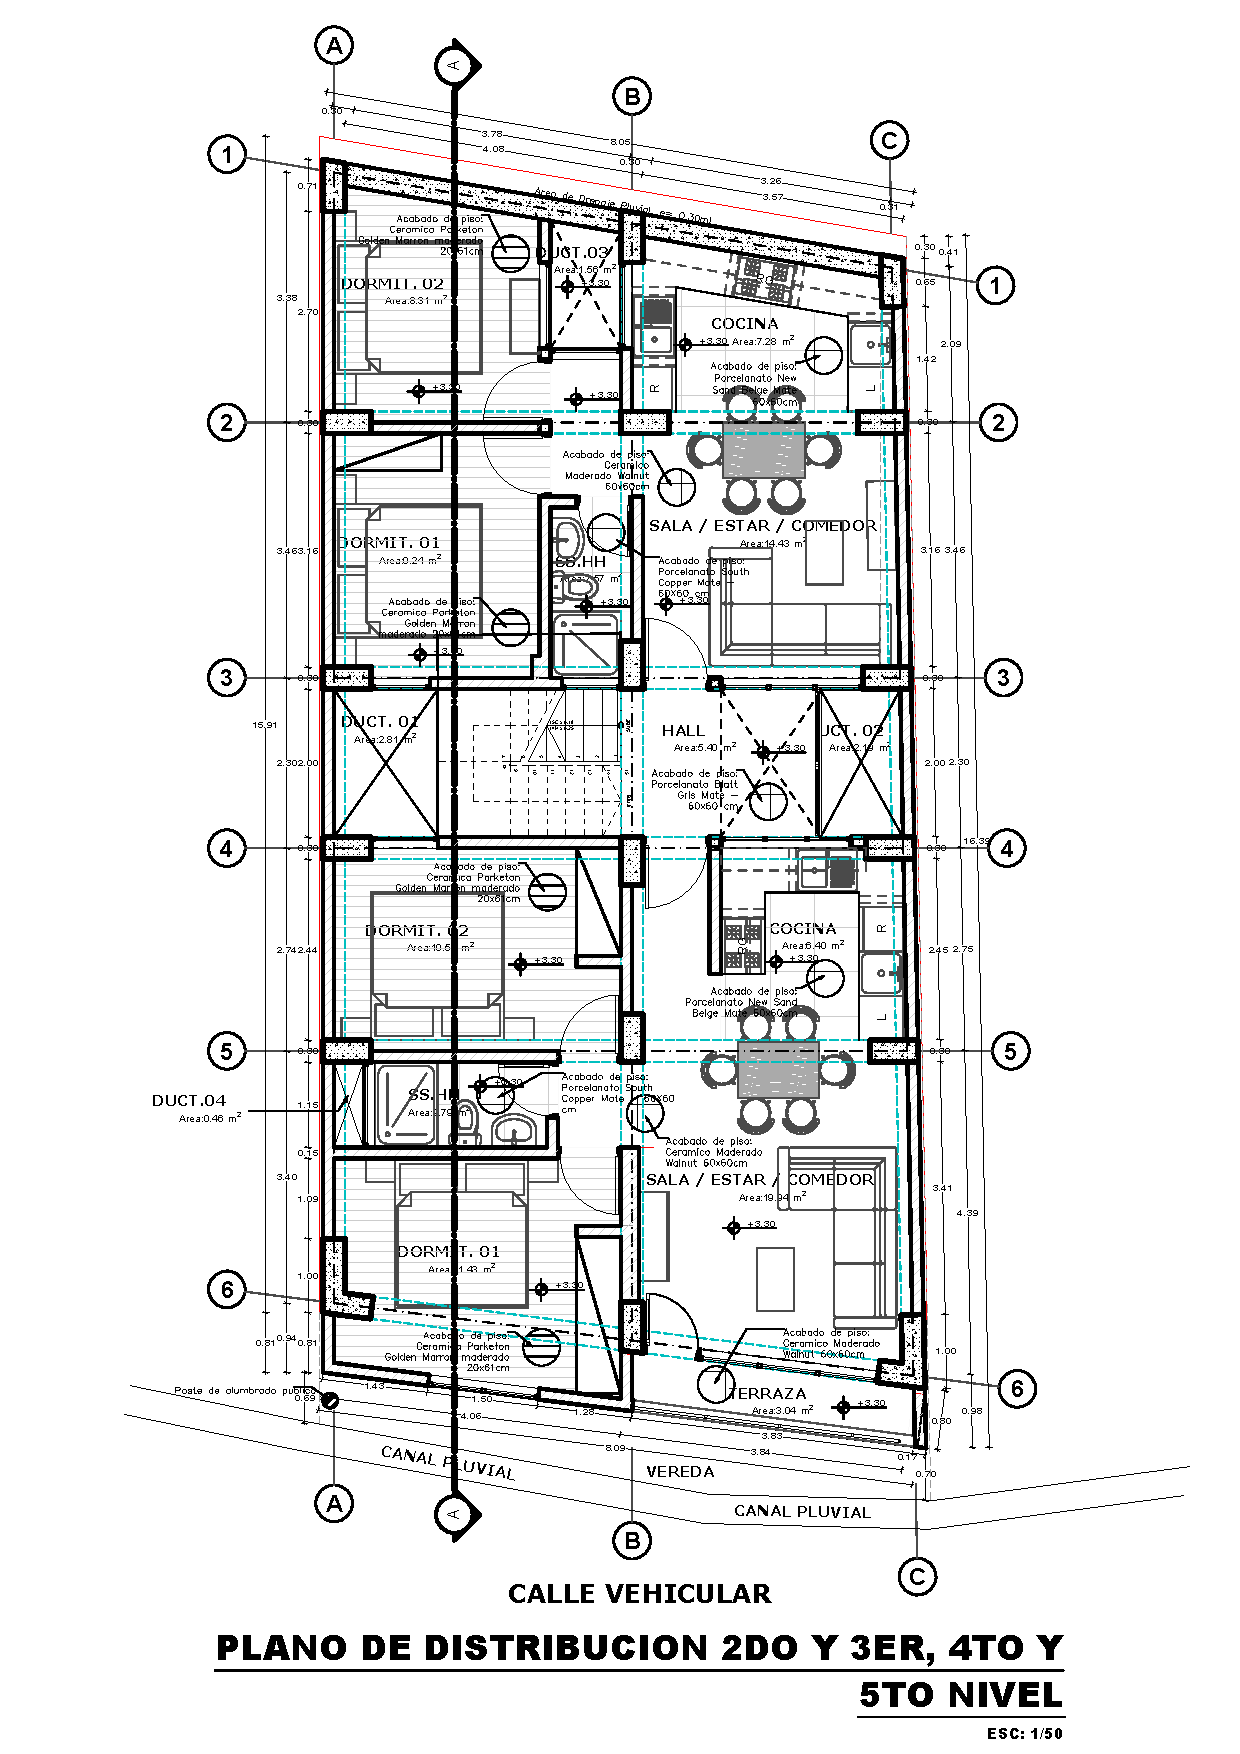
\includegraphics[scale=0.7]{IMAGENES/Plano.pdf}
    \label{pl}
\end{figure}

\begin{figure}[ht!]
    \centering
    \caption{Elevación}
    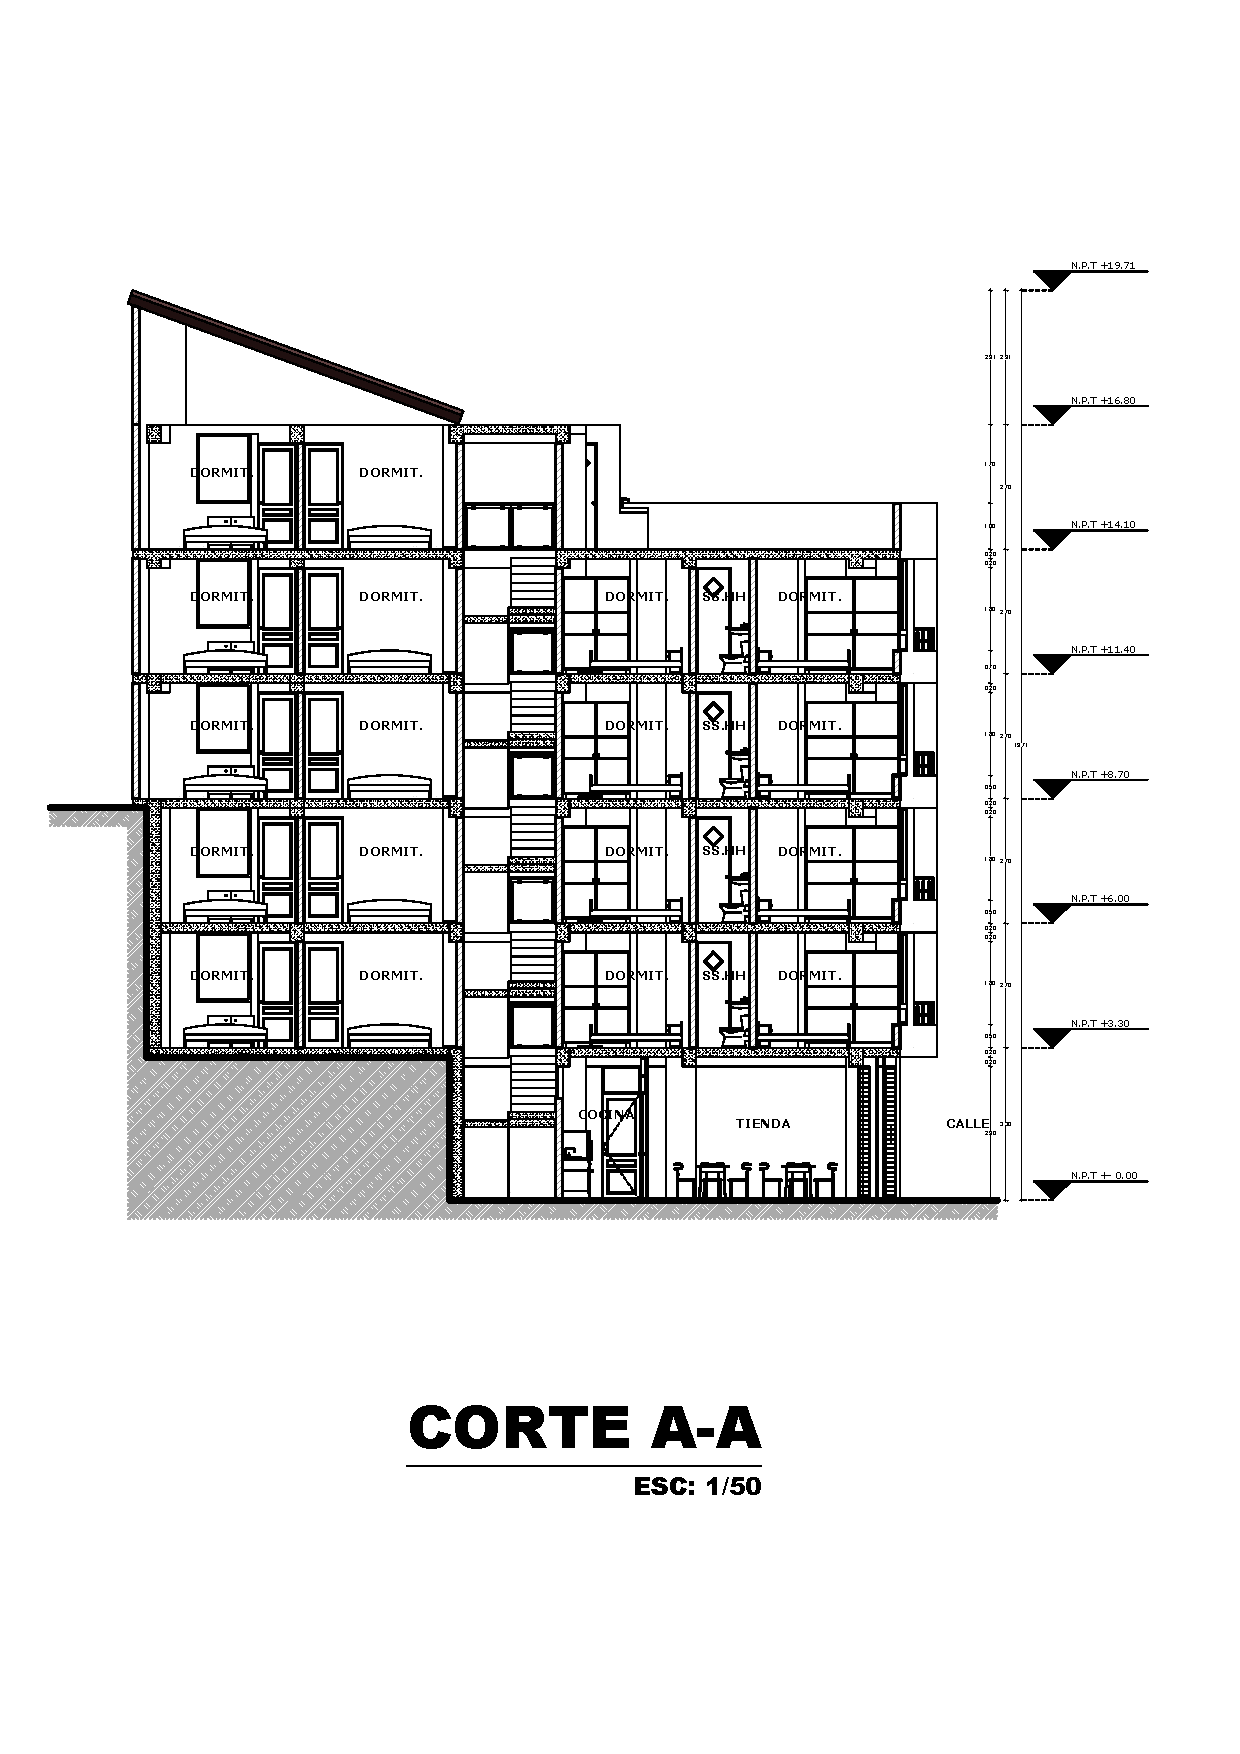
\includegraphics[trim={0 2cm 0 4.2cm},scale=0.7]{IMAGENES/ele.pdf}
    \label{el}
\end{figure}
%trim={<izquierda> <abajo> <derecha> <arriba>}
\section{Bases legales}
El desarrollo del presente trabajo se basa en las siguientes normas y reglamentos:
\begin{itemize}
  \item Norma Técnica de Edificación E.020 (Cargas)
  \item Norma Técnica de edificación E.030 (Diseño Sismoresistente)
  \item Norma Técnica de edificación E.050 (Suelos y Cimentaciones)
  \item Norma Técnica de edificación E.060 (Concreto Armado)
\end{itemize}

\section{Cargas de diseño}
Los cálculos y las consideraciones propias para el análisis con cargas de gravedad y de sismo, así como el diseño estructural del edificio se realizarán de acuerdo a lo especificado en las normas NTE E-020 Metrado de Cargas, NTE E-030 Diseño Sismorresistente, NTE E-060 Diseño de Concreto Armado.

\subsection{Cargas Muertas}

Las cargas muertas se determinan del cálculo directo del peso de todos los componentes estructurales y de elementos no estructurales cuya posición no se modificará durante la vida útil de la edificación. La norma E-020 del RNE nos proporciona algunos pesos unitarios para calcular la carga muerta, en nuestro caso tenemos:
\vspace{0.8cm}
% Table generated by Excel2LaTeX from sheet 'Hoja1'
\begin{table}[htbp]
  \centering
 % \caption{Add caption}
    \begin{tabular}{lrl}
    Concreto armado & :     & 2400 kg/m\raisebox{1ex}{\scriptsize{3}}\\
              &       &  \\
    Muro de albañilería hueca & :     & 1350 kg/m\raisebox{1ex}{\scriptsize{3}} \\
              &       &  \\
    Muro de albañilería solida                              & :     & 1800 kg/m\raisebox{1ex}{\scriptsize{3}}  \\
              &       &  \\
    Mortero de cemento & :     & 2000 kg/m\raisebox{1ex}{\scriptsize{3}}  \\
              &       &  \\
    Piso terminado (pt)  & :     & 100 kg/m\raisebox{1ex}{\scriptsize{2}}  \\
    \end{tabular}%
  \label{tab:addlabel}%
\end{table}%

La carga muerta lo calcula el programa, pero adicionalmente se consideró una sobrecarga permanente de 100 kg/m\raisebox{1ex}{\scriptsize{2}} que incluye piso terminado.
También se incluyó las cargas distribuidas directamente sobre vigas debido a las tabiquerías de espesor 15 cm. Los muros se suponen construidos con ladrillos pandereta cuyo peso especifico se extrae de la norma E-020:

\begin{figure}[h!]
    \centering
    \caption{Peso unitario de tabiquería}
    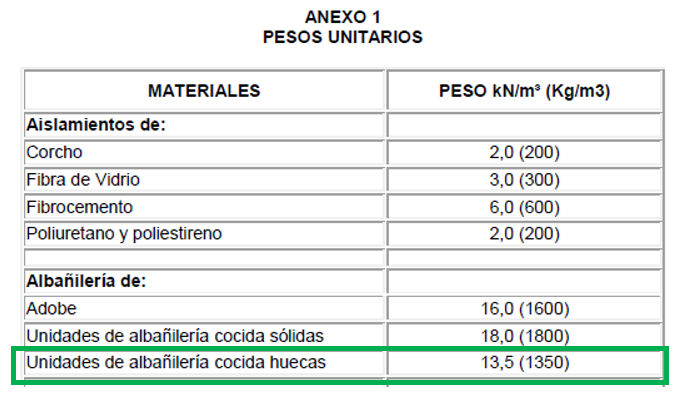
\includegraphics[scale=0.7]{IMAGENES/3.PNG}
    \caption*{\small Fuente: \it \cite{E-020}}
    \label{fig:my_label}
\end{figure}

\newpage

\subsection{Cargas Vivas}
La carga de piso que se va aplicar a un área determinada de una edificación depende de su pretendida utilización u ocupación. Estas cargas se deben a los seres humanos, al equipo, al almacenamiento en general, a los automóviles, etc., debido a que estas cargas son de naturaleza aleatoria, no hay una forma precisa para aplicar las cargas reales a un área dada. Por esa razón se especifican como cargas distribuidas uniformemente en el área. Cabe indicar que estas cargas son extremamente conservadoras debido a la incertidumbre acerca de cómo pudieran distribuirse las cargas reales. La norma E020 nos da cargas distribuidas para distintos tipos de ocupación o uso, en nuestro caso para una edificacion de vivienda se tiene:  

\begin{figure}[h]
    \centering
    \caption{Carga viva para viviendas}
    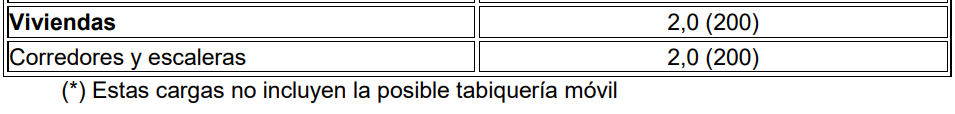
\includegraphics[scale=0.8]{IMAGENES/4.PNG}
    \label{fig:my_label}
    \caption*{\small Fuente: \it \cite{E-020}}
\end{figure}

\begin{figure}[h]
    \centering
    \caption{Carga viva en azoteas}
    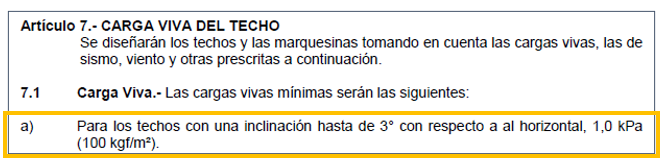
\includegraphics[scale=1]{IMAGENES/7.PNG}
    %\label{fig:my_label}
    \caption*{\small Fuente: \it \cite{E-020}}
\end{figure}

\newpage
\section{Propiedades del material}

Dado que se trata de un análisis lineal elástico las únicas propiedades que involucran en el calculo son las del concreto y se extraen de la \cite{E-060}:
\vspace{0.5cm}
% Table generated by Excel2LaTeX from sheet 'Hoja1'
\begin{table}[htbp]
  \centering
 % \caption{Add caption}
    \begin{tabular}{>{\arraybackslash}m{7cm}>{\arraybackslash}m{0.2cm}>{\arraybackslash}m{8cm}}
    $\bullet$ Resistencia máxima a la compresión  & :     & $f' _{c}=210$ kg/cm\raisebox{1ex}{\scriptsize{2}} \\
              &       &  \\
   % $\bullet$ Deformación unitaria máxima  & :     & $\varepsilon _{c}=0.003$ \\
   %           &       &  \\
    $\bullet$ Módulo de Elasticidad  & :     & $E _{c}=15000\;f'_{c}=217,370.65
    $ kg/cm\raisebox{1ex}{\scriptsize{2}} \\
              &       &  \\
    $\bullet$ Relación entre módulos de elasticidad & :     & $E _{c}/G=2.3$ \\
    \end{tabular}%
  \label{tab:addlabel}%
\end{table}%

\section{Estructuracion}
Según \cite{san1998analisis}, la estructuración de un edificio consiste en “tomar decisiones en conjunto con los otros profesionales que intervienen en la obra acerca de la disposición y características que deben tener los diferentes elementos estructurales, de manera que el edificio tenga un buen comportamiento durante su vida útil; esto es, que tanto las cargas permanentes (peso propio, acabados, etc.) como las eventuales (sobrecarga, sismo, viento, etc.), y se transmitan adecuadamente hasta el suelo de cimentación”.\\
\section{Predimensionamiento}
\subsection{Losas Aligeradas}
Según \cite{blanco} el peralte de las losas aligeradas podrá ser dimensionado considerando los siguientes criterios:
\newpage
\begin{table}[htbp]
  \centering
  \caption{Peso propio y espesores recomendados en aligerados}
  \vspace{0.15cm}
{
\extrarowheight = -0.5ex
\renewcommand{\arraystretch}{1.8}

\begin{tabular}{|>{\centering\arraybackslash}m{2cm}|>{\centering\arraybackslash}m{5cm}| >{\centering\arraybackslash}m{5cm}|}
 %\begin{tabular}{|c|c|c|}
    \hline
    \textbf{h (m)} & 
    \textbf{Peso propio aproximado (kg/m\raisebox{1ex}{\scriptsize{2}})} & 
    \textbf{Luces máximas recomendadas (m)} \\
    \hline
    0.17  & 280   & ln $\leq$ 4 \\
    0.20   & 300   & 4 $\leq$ ln $\leq$ 5.5 \\
    0.25  & 350   & 5.5 $\leq$ ln $\leq$ 6.6 \\
    0.30   & 420   & 6 $\leq$ ln $\leq$ 7.5 \\
    \hline
 \end{tabular}%
}
  \caption*{\small Fuente: \it \cite{blanco}}
  \label{tab:addlabel}%
\end{table}%
\noindent
Se entiende por h al espesor total del aligerado incluyendo los 5cm de losa superior.
\\
El criterio anterior sólo aplica para sobrecargas máximas de 300 a 350 kg/m\raisebox{1ex}{\scriptsize{2}}.
\\
Teniendo en cuenta estos criterios se adopto losas aligeradas armadas en el sentido paralelo a los ejes A,B y C. El espesor entre los ejes 1 y 3 es de 17cm y entre los ejes 4 y 6 es de 20cm.

\subsection{Losas Macizas}
Se adopto una losa maciza en la zona donde existe discontinuidad del diafragma debido a los ductos y la presencia de la escalera. Se adopto un peralte de 20cm con la intención de trasmitir las fuerzas sísmicas del diafragma adecuadamente a los demás elementos.

\subsection{Vigas principales}
Se provee al edificio de vigas peraltadas en las dos direcciones ``X'' e ``Y'', a manera de contar con suficiente rigidez lateral ante un evento sísmico y trabajen de manera conjunta como pórtico y/o pórtico-placa.
\\
Según \cite{blanco}, las vigas se dimensionan generalmente considerando un peralte del orden de 1/10 a 1/12 de la luz libre.
\\
Las vigas dimensionadas con este criterio son diseñadas solo con acero en tracción y no existe problemas de deflexiones grandes.
La norma peruana E 060 indica que el ancho mínimo de vigas que forman parte de elementos sismorresistentes debe ser 25cm.
\\
Las luces libres de máxima longitud son de aproximadamente de 4m por lo que según este criterio solo sería necesario peraltes del orden de 40cm, sin embargo, después de realizar el análisis sísmico se adoptó vigas principales de 30x50cm para cumplir con los requisitos que se mencionan posteriormente.

\subsection{Vigas secundarias}
Al igual que en el caso anterior las dimensiones finales de las vigas secundarias son por requerimiento de rigidez lateral resultando estas 25x40cm.

\subsection{Columnas}

Según \cite{ovi2016} las dimensiones de las columnas se pueden estimar con la expresión:

\begin{equation}
A_{c}=\frac{\lambda\;P_{g} }{\eta \;f'_{c}}
\end{equation}
\myequations{Predimensonamiento de columnas}

\begin{flushleft}
Donde:\\
$\lambda$, $\eta$ = Factores obtenidos de la tabla .\\
$P_{g}$ = Carga gravitacional repartida por m\raisebox{1ex}{\scriptsize{2}}, se puede asumir 1 ton/m\raisebox{1ex}{\scriptsize{2}}\\
$f'_{c}$ = Resistencia a compresión del concreto.\\
\end{flushleft}

% Table generated by Excel2LaTeX from sheet 'Hoja1'
\begin{table}[htbp]
  \centering
  \caption{Predimensionamiento de columnas}
    \begin{tabular}{|c|c|c|}
    \hline
    \rowcolor[rgb]{ .906,  .902,  .902} \textit{\textbf{Tipo de columna:}} & \multicolumn{1}{p{10.665em}|}{\centering\textbf{$\lambda$}} & \multicolumn{1}{p{11.945em}|}{\centering\textbf{$\eta$}} \\
    \hline
    \rowcolor[rgb]{ .906,  .902,  .902} Central & \cellcolor[rgb]{ 1,  1,  1}1.10 & \cellcolor[rgb]{ 1,  1,  1}0.30 \\
    \hline
    \rowcolor[rgb]{ .906,  .902,  .902} Perimetral & \cellcolor[rgb]{ 1,  1,  1}1.25 & \cellcolor[rgb]{ 1,  1,  1}0.25 \\
    \hline
    \rowcolor[rgb]{ .906,  .902,  .902} Esquinera & \cellcolor[rgb]{ 1,  1,  1}1.50 & \cellcolor[rgb]{ 1,  1,  1}0.20 \\
    \hline
    \end{tabular}%
  \label{tab:addlabel}%
\end{table}%

Después de aplicar la ecuación  para la columnas con mayor área tributaria se obtuvo dimensiones mínimas, sin embargo las dimensiones finales de las columnas son por requerimiento de rigidez lateral, resultado estas de 30x65 peraltadas en la dirección paralela al eje X.


\subsection{Muros de corte o placas}

La longitud final de los muros en ambas direcciones se establece después de realizar un análisis sísmico iterativo hasta cumplir con los requisitos de rigidez lateral de la norma E-030.

\section{Modelamiento}

El modelo matemático se construyo en el software de análisis y diseño estructural ETABS en su versión 20.1.1, el material se definió según lo mencionado en el inciso 7 del presente documento, las secciones se crearon según lo mencionado en el predimensionamiento. Para el modelado de losas y muros se utilizo elementos shell y para columnas y vigas se utilizo elementos frame, sin embargo cuando existe columnas que forman parte de algún muro estos se modelaron con elementos shell para integrar de mejor manera los esfuerzos resultantes, asi mismo se aseguro un correcto mesh en esos elementos para poder capturar el comportamiento a flexion. 
\\
Las alturas de entrepiso se tomaron según los planos de arquitectura, la profundidad de cimentación se considero de 3.10m y las columnas y muros se modelaron hasta la cara superior de la cimentación, para lo cual se estimo un espesor de la zapata o platea de 0.6m. 
\\
Las zonas de los nudos de columnas y vigas se modelaron con un factor de rigidez del 50 \%, se consideran las rigideces brutas de los elementos como se menciona en la E-030 a excepción de las losas donde se redujo la rigidez axial, a flexión y a cortante a un 25 \% según lo mencionado en \cite{ACI19}. Debido a las aberturas y la relación de dimensiones de la planta del edificio no se considera un diafragma rígido en los sistemas de piso.
\\
\newpage

\newsavebox\mybox
\savebox{\mybox}{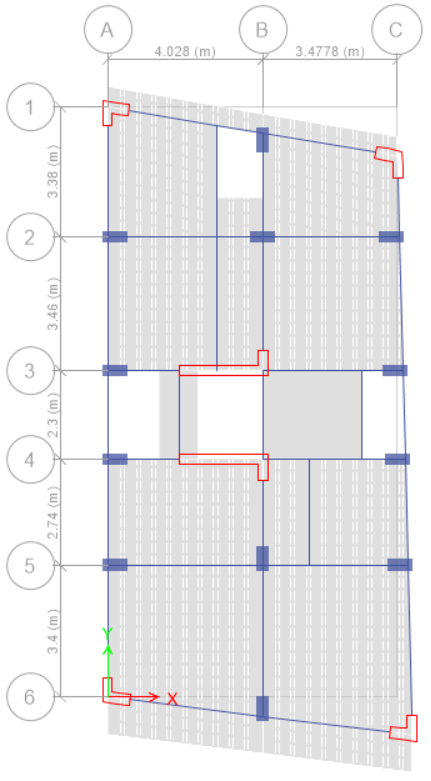
\includegraphics[width=7cm]{IMAGENES/6.PNG}}
\begin{figure}[h]
    \centering
    \begin{minipage}{0.45\textwidth}
        \centering
        \usebox{\mybox}
        \caption{Planta típica}
    \end{minipage}
    \begin{minipage}{0.45\textwidth}
        \centering
        \vbox to \ht\mybox{%
            \vfill
            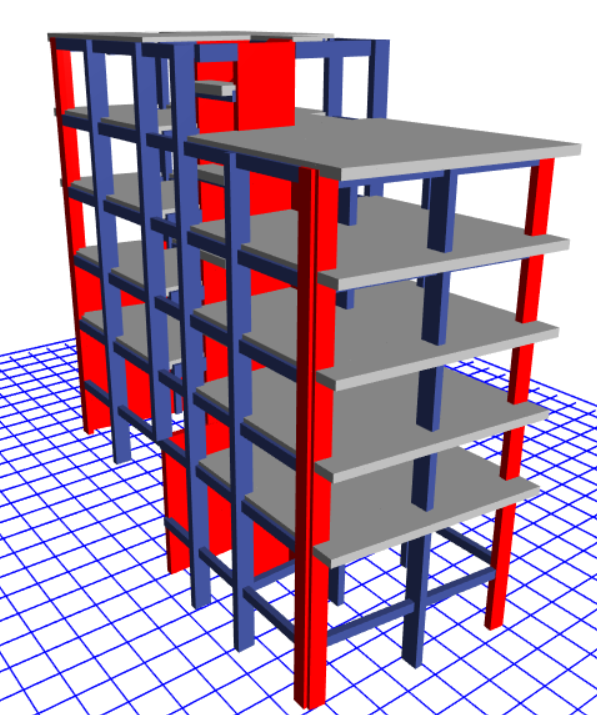
\includegraphics[width=7cm]{IMAGENES/5.PNG}
            \vfill
        }
        \caption{Vista 3D}
    \end{minipage}
\end{figure}

\section{Análisis Sísmico}
\subsection{Parámetros de sitio}
\subsubsection{Zonificación}
La ubicación de este proyecto es en la ciudad de Cusco, en el distrito de Cusco. Siguiendo los parámetros de la norma de diseño sismorresistente E.030 de octubre de 2018, la estructura se encuentra en la Zona 2. Por ello que el factor que se interpreta como la aceleración máxima horizontal en el suelo rígido con una probabilidad de 10 \% de ser excedida en 50 años es igual a \textbf{0.25}.
\newpage
%\vspace{-10cm}
\begin{table}[ht!]
    \centering
    \begin{minipage}{0.55\textwidth}
    \vspace{-4cm}
    \caption{Factor de zona}
    \begin{tabular}{|>{\centering\arraybackslash}m{3.75cm}|>{\centering\arraybackslash}m{3.75cm}|}
    \hline
    \multicolumn{2}{|c|}{\textbf{FACTOR DE ZONA SEGÚN E-030}} \\
    \hline
    \textit{\textbf{ZONA}} & \textit{\textbf{Z}} \\
    \hline
    4     & 0.45 \\
    \hline
    3     & 0.35 \\
    \hline
    \rowcolor[rgb]{ .949,  .949,  .949} 2     & \textcolor[rgb]{ 1,  0,  0}{\textbf{0.25}} \\
    \hline
    1     & 0.10 \\
    \hline
    \end{tabular}%
    \end{minipage}
    \begin{minipage}{0.35\textwidth}
    \vspace{-4cm}
        \centering
        \vbox to \ht\mybox{%
            \vfill
            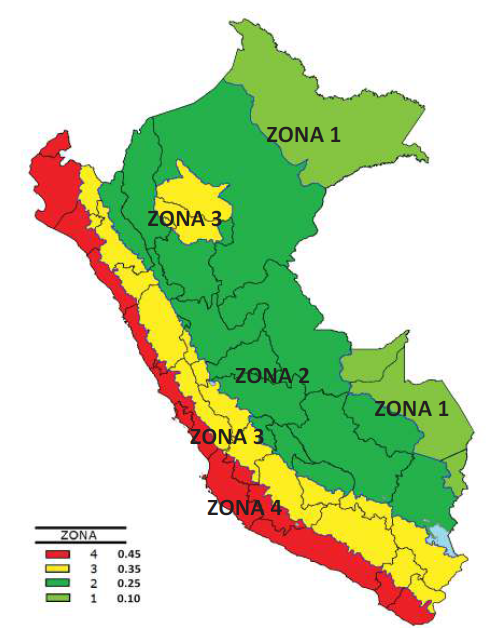
\includegraphics[width=4cm]{IMAGENES/8.png}
            \vfill
        }
    \end{minipage}
    \vspace{-3.5cm}
    \caption*{\small Fuente: \it \cite{E-030}}
\end{table}
%\vspace{-3.5cm}
\subsubsection{Factor de suelo}
%\vspace{-4cm}
% Table generated by Excel2LaTeX from sheet '00-d) Parametros sismicos'
\begin{table}[h!]
  \centering
  \caption{Factor de suelo}
    \begin{tabular}{|>{\centering\arraybackslash}m{3.75cm}|>{\centering\arraybackslash}m{2cm}|>{\centering\arraybackslash}m{2cm}|>{\centering\arraybackslash}m{2cm}|>{\centering\arraybackslash}m{2cm}|}
    \hline
    \multicolumn{5}{|c|}{\textbf{FACTOR DE SUELO SEGÚN E-030}} \\
    \hline
    \backslashbox{\textit{\textbf{ZONA}}}{\textit{\textbf{SUELO}}} & \textit{\textbf{S0}} & \textit{\textbf{S1}} & \textit{\textbf{S2}} & \textit{\textbf{S3}} \\
    \hline
    \textit{\textbf{4}} & 0.80  & 1.00  & 1.05  & \cellcolor[rgb]{ .949,  .949,  .949}1.10 \\
    \hline
    \textit{\textbf{3}} & 0.80  & 1.00  & 1.15  & \cellcolor[rgb]{ .949,  .949,  .949}1.20 \\
    \hline
    \rowcolor[rgb]{ .949,  .949,  .949} \textit{\textbf{2}} & 0.80  & 1.00  & 1.20  & \textcolor[rgb]{ 1,  0,  0}{\textbf{1.40}} \\
    \hline
    \textit{\textbf{1}} & 0.80  & 1.00  & 1.60  & \cellcolor[rgb]{ .949,  .949,  .949}2.00 \\
    \hline
    \end{tabular}%
    \caption*{\small Fuente: \it \cite{E-030}}
  \label{tab:addlabel}%
\end{table}%

\subsubsection{Periodos de suelo}
% Table generated by Excel2LaTeX from sheet '00-d) Parametros sismicos'
\begin{table}[h!]
  \centering
  \caption{Periodos de suelo}
    \begin{tabular}{|>{\centering\arraybackslash} m{2cm}|>{\centering\arraybackslash}m{2cm}|>{\centering\arraybackslash}m{2cm}|>{\centering\arraybackslash}m{2cm}|>{\centering\arraybackslash}m{2cm}|}
\cline{2-5}     \multicolumn{1}{r|}{} & \multicolumn{4}{c|}{\textbf{PERIODO "Tp" y "Tl" SEGÚN E-030}} \\
\cline{2-5}     \multicolumn{1}{r|}{} & \multicolumn{4}{c|}{\textit{\textbf{Perfil de suelo}}} \\
\cline{2-5}     \multicolumn{1}{r|}{} & \textit{\textbf{S0}} & \textit{\textbf{S1}} & \textit{\textbf{S2}} & \textit{\textbf{S3}} \\
    \hline
    \textit{\textbf{Tp}} & 0.30  & 0.40  & 0.60  & \cellcolor[rgb]{ .949,  .949,  .949}\textcolor[rgb]{ 1,  0,  0}{\textbf{1.00}} \\
    \hline
    \textit{\textbf{Tl}} & 3.00  & 2.50  & 2.00  & \cellcolor[rgb]{ .949,  .949,  .949}\textcolor[rgb]{ 1,  0,  0}{\textbf{1.60}} \\
    \hline
    \end{tabular}%
    \caption*{\small Fuente: \it \cite{E-030}}
  \label{tab:addlabel}%
\end{table}%

\subsection{Sistema Estructural}
Después de realizar el análisis sísmico se determino que los sistemas estructurales en X, Y son de muros y pórticos respectivamente.
% Table generated by Excel2LaTeX from sheet '00-d) Parametros sismicos'
\begin{table}[h!]
  \centering
  \caption{coeficiente básico de reducción }
    {
\extrarowheight = -0.3ex
\renewcommand{\arraystretch}{1.4}
    \begin{tabular}{|>{\arraybackslash}m{10cm}| >{\centering\arraybackslash}m{4cm}|}
    \hline
    \multicolumn{2}{|c|}{\textbf{SISTEMAS ESTRUCTURALES }} \\
    \hline
    \textit{\textbf{Sistema Estructural}} & \multicolumn{1}{m{4cm}|}{\textit{\textbf{Coeficiente Básico de Reducción Ro}}} \\
    \hline
    \multicolumn{2}{|l|}{\textbf{Acero:}} \\
    \hline
    Porticos Especiales Resistentes a Momento (SMF) & 8 \\
    \hline
    Porticos Intermedios Resistentes a Momento (IMF) & 5 \\
    \hline
    Porticos Ordinarios Resistentes a Momento (OMF) & 4 \\
    \hline
    Porticos Especiales Concentricamente Arrriostrados (SCBF) & 7 \\
    \hline
    Porticos Ordinarios Concentricamente Arrriostrados (OCBF) & 4 \\
    \hline
    Porticos Excentricamente Arriostrados (EBF) & 8 \\
    \hline
    \multicolumn{2}{|l|}{\textbf{Concreto Armado:}} \\
    \hline
    \rowcolor[rgb]{ .906,  .902,  .902} Porticos & \textcolor[rgb]{ 1,  0,  0}{\textbf{8}} \\
    \hline
     Dual  & 7 \\
    \hline
    \rowcolor[rgb]{ .906,  .902,  .902} De muros estructurales & \textcolor[rgb]{ 1,  0,  0}{\textbf{6}} \\
    \hline
    Muros de ductilidad limitada & 4 \\
    \hline
    \textbf{Albañilería Armada o Confinada} & 3 \\
    \hline
    \textbf{Madera} & 7 \\
    \hline
    \end{tabular}%
    }
    \caption*{\small Fuente: \it \cite{E-030}}
  \label{tab:addlabel}%
\end{table}%
\vspace{-0.8cm}

\subsection{Factor de amplificación sísmica}
Se determina según el articulo 11 de la E-030.
\newpage
%\newpage
\setlength{\jot}{0.5cm}% Inter-equation spacing
\begin{figure}[h!]
    \centering
    \begin{minipage}{0.5\textwidth}
    \vspace{-4cm}
    \caption{Factor de amplificación}
        \begin{align*}
        &T< T_{P}         &   C&=2,5\cdot\left ( \frac{T_{P}}{T} \right )\\
        &T_{P}< T< T_{L}  &   C&=2,5\cdot\left ( \frac{T_{P}}{T} \right )\\
        &T> T_{L}         &   C&=2,5\cdot\left ( \frac{T_{P}\;T_{L}}{T^{2}} \right )
        \end{align*}
    \end{minipage}
    \begin{minipage}{0.4\textwidth}
    \vspace{-3cm}
        \centering
        \vbox to \ht\mybox{%
            \vfill
            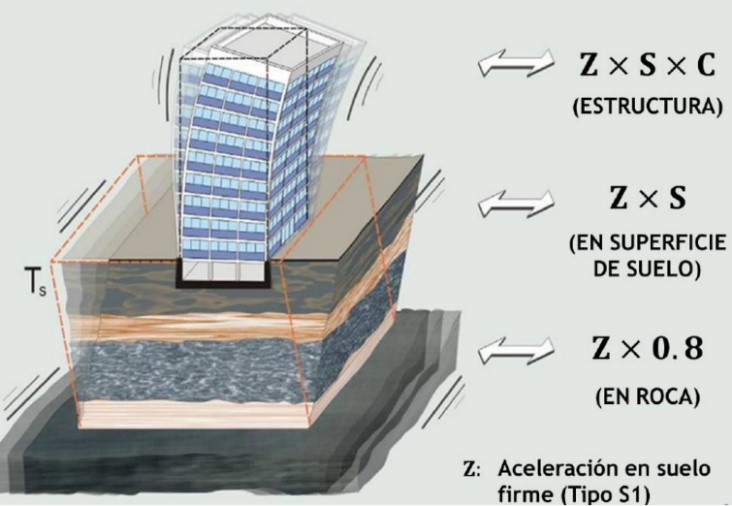
\includegraphics[width=6.5cm]{IMAGENES/9.jpg}
            \vfill
       }
    \end{minipage}
    \vspace{-3.4cm}
    \caption*{\small Fuente: \it \cite{comen}}
  \label{fac}
\end{figure}
\vspace{-0.8cm}
\subsection{Factor de importancia}
% Table generated by Excel2LaTeX from sheet '00-d) Parametros sismicos'
\begin{table}[h!]
  \centering
  \caption{Factor de Uso o importancia}
    \begin{tabular}{|>{\arraybackslash}m{3cm}|m{8cm}|>{\arraybackslash}m{2.8cm}|}
    \hline
    \multicolumn{3}{|c|}{\textbf{CATEGORIA DE LA EDIFICACION}} \\
    \hline
    \multicolumn{1}{|c|}{\textit{\textbf{CATEGORIA}}} & \multicolumn{1}{c|}{\textit{\textbf{DESCRIPCION}}} & \multicolumn{1}{c|}{\textit{\textbf{FACTOR U}}} \\
    \hline
    \multirow{2}[4]{3cm}{A Edificaciones Escenciales} & A1: Establecimiento del sector salud (públicos y privados) del segundo y tercer nivel, según lo normado por el ministerio de salud. & Con aislamiento 1.0 y sin aislamiento 1.5. \\
\cline{2-3}    \multicolumn{1}{|c|}{} & A2: Edificaciones escenciales para el manejo de las emergencias, el funcionamiento del gobierno y en general aquellas que puedan servir de refugio después de un desastre. & \multicolumn{1}{c|}{1.50} \\
    \hline
    B Edificaciones Importantes & Edificaciones donde se reúnen gran cantidad de personas tales como cines, teatros, estadios, coliseos, centros comerciales, terminales de buses de pasajeros, establecimientos penitenciarios, o que guardan patrimonios valiosos como museos y bibliotecas. & \multicolumn{1}{c|}{1.30} \\
    \hline
    \rowcolor[rgb]{ 1,  .949,  .8} C Edificaciones Comunes & Edificaciones comunes tales como: viviendas, oficinas, hoteles, restaurantes, depósitos e instalaciones industriales cuya falla no acarree peligros adicionales de incendios o fugas de contaminantes. & \multicolumn{1}{c|}{\textcolor[rgb]{ 1,  0,  0}{\textbf{1.00}}} \\
    \hline
    D Edificaciones temporales & Construcciones provisionales para depósitos, casetas y otras similares. & A criterio del proyectista \\
    \hline
    \end{tabular}%
    \caption*{\small Fuente: \it \cite{E-030}}
  \label{tab:addlabel}%
\end{table}%


\newpage


% Table generated by Excel2LaTeX from sheet '07) ESPECTRO FINAL'
\begin{table}[htbp]
  \centering
  \caption{Resumen de parámetros sísmicos}
  {
\extrarowheight = -0.3ex
\renewcommand{\arraystretch}{1.5}
    \begin{tabular}{m{5cm}|>{\centering\arraybackslash}m{2cm}|>{\centering\arraybackslash}m{2cm}|>{\centering\arraybackslash}m{2cm}|}
\cline{2-4}          & \multicolumn{3}{c|}{\textbf{PARAMETROS SISMICOS}} \\
\cline{2-4}          &       & \textit{\textbf{X}} & \textit{\textbf{Y}} \\
\cline{2-4}  \multicolumn{1}{l|}{\textit{Factor de Zona (Tabla N°1)}} & \textbf{Z} & \multicolumn{2}{c|}{0.25} \\
\cline{2-4}    \multicolumn{1}{l|}{\textit{Factor de Uso (Tabla N°5)}} & \textbf{U} & \multicolumn{2}{c|}{1.00} \\
\cline{2-4}    \multicolumn{1}{l|}{\textit{Factor de Suelo (Tabla N°3)}} & \textbf{S} & \multicolumn{2}{c|}{1.40} \\
\cline{2-4}    \multicolumn{1}{l|}{\multirow{2}{*}{\textit{Periodos (Tabla N°4)}}} & \textbf{T\raisebox{-0.5ex}{\scriptsize{P}}} & \multicolumn{2}{c|}{1.00} \\
\cline{2-4}          & \textbf{T\raisebox{-0.5ex}{\scriptsize{L}}} & \multicolumn{2}{c|}{1.60} \\
\cline{2-4}    \multicolumn{1}{l|}{\textit{Coef. Básico de Reducción (Tabla N°7)}} & \textbf{R\raisebox{-0.5ex}{\scriptsize{o}}} & 6.00  & 8.00 \\
\cline{2-4}    \multicolumn{1}{l|}{\textit{Irregularidad en altura (Tabla N°8)}} & \textbf{I\raisebox{-0.5ex}{\scriptsize{a}}} & 1.00  & 1.00 \\
\cline{2-4}    \multicolumn{1}{l|}{\textit{Irregularidad en planta (Tabla N°9)}} & \textbf{I\raisebox{-0.5ex}{\scriptsize{p}}} & 1.00  & 1.00 \\
\cline{2-4}    \multicolumn{1}{l|}{\textit{Coef. de Reducción (Articulo 22)}} & \textbf{R} & 6.00  & 8.00 \\
\cline{2-4}          & \textbf{ZUSg/R} & 0.57  & 0.43 \\
\cline{2-4}    \end{tabular}%
}
  \label{tab:addlabel}%
\end{table}%

\subsection{Espectro de respuesta de aceleraciones}
\begin{figure}[h!]
    \centering
    \begin{tikzpicture}
    %draw[color=blue, help lines,dashed ] (0,0) grid (4.5,1.7);
    \begin{axis}
    [grid=both,
    grid style={line width=.1pt,dashed, draw=gray!10},
    major grid style={line width=.2pt,draw=gray!50},name=plot, xlabel={T (s)},ylabel={Sa (m/s2)},xmin=0,xmax=4,
    ymin=0,ymax=1.7,width=.8\textwidth,height=10cm,legend entries={X (R=6),Y(R=8)},legend pos=north east]%,xtick distance=.5%,ytick distance=.5]
    \addplot[OrangeRed,ultra thick] table{./EX6.txt};\label{xx}
    \addplot[MidnightBlue,ultra thick] table{./EY8.txt};\label{yy}
    %\addplot[black,mark=triangle*] table{./espectro R=8.txt};\label{f}
    %\addplot[red,mark=o] table{./data/generator.txt};\label{g}
    %\addplot[blue] table{./data/simulated_total.txt};\label{s}
    %\addplot[green,dashed] table{./data/theoretical_total.txt};\label{t}
% Define two points for drawing an arrow to the "matched" point
    \node[] (C) at (axis cs: 1,1.6) {\hspace{0.5cm}Tp};
    \node[] (B) at (axis cs: 1,0) {};
    \node[] (D) at (axis cs: 1.6,1.6) {\hspace{0.5cm}Tl};
    \node[] (G) at (axis cs: 1.6,0) {};
    \end{axis}
 % Create a node to act as the legend  
    %\node[anchor=north,fill=white,draw=black] (legend) at ($(plot.north)-(-28 mm, 8.5 mm)$) {\begin{tabular}{l l l l}
       % X (R=6) & \ref{xx}\\ % & Y (R=8) & \ref{yy} \\
       % Y (R=8) & \ref{yy}\\ % & Y (R=8) & \ref{yy} \\
        %s & \ref{s}  & t & \ref{t} \\
   % \end{tabular} };

%\draw [dashed] (10,1) -- (10,11);
\draw[dashed,color=green,line width=1pt] (C)--(B);
\draw[dashed,color=orange,line width=1pt] (D)--(G);
%\node[anchor=west] (label) at (B) {matched};
    
    \end{tikzpicture}
    \caption{Espectro de aceleraciones}
    \label{fig:my_label}
\end{figure}


\subsection{Peso Sísmico}
\begin{mybox3}{Art. 23 E-030}
\textit{El peso (P), se calcula adicionando a la carga permanente y total de la edificación un porcentaje de la carga viva o sobrecarga. En edificaciones de la categoría C, se toma el 25\% de la carga viva.}
\end{mybox3}

\subsection{Excentricidad Accidental}

\begin{mybox3}{Art. 26.5 E-030}
\textit{La incertidumbre en la localización de los centros de masa en cada nivel, se considera mediante una excentricidad accidental perpendicular a la dirección del sismo igual a 0,05 veces la dimensión del edificio en la dirección perpendicular a la dirección de análisis. En cada caso se considera el signo más desfavorable.}
\end{mybox3}
\noindent
Para determinar el sentido mas desfavorable de la excentricidad accidental se calculo el centro de masa y centro de rigidez del edificio, resultando negativo en ambos casos, la excentricidad se asigna a la masa como se muestra en la figura \ref{masa} .

\begin{figure}[h!]
    \centering
    \caption{Excentricidad de la masa en ETABS}
    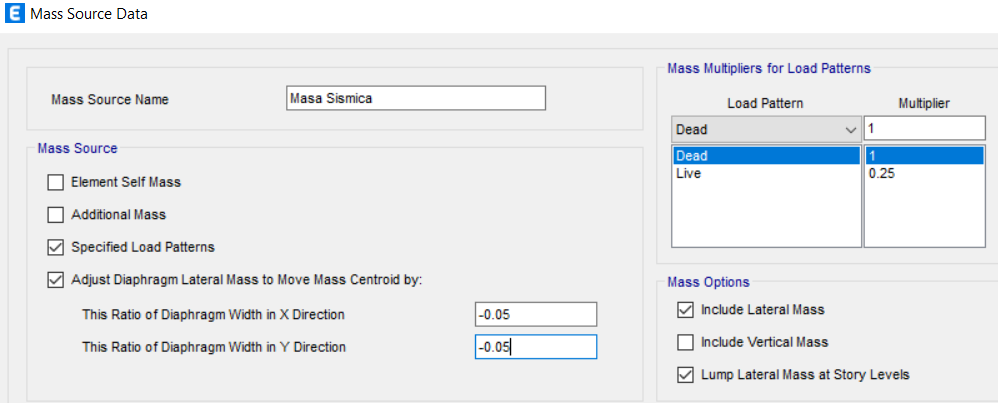
\includegraphics[scale=0.7]{IMAGENES/15.PNG}
    \label{masa}
\end{figure}

\newpage
\subsection{Análisis modal Art. 26.1 E-030}

\begin{mybox3}{Art. 26.1.1}
\textit{Los modos de vibración pueden determinarse por un procedimiento de análisis que considere apropiadamente las características de rigidez y la distribución de las masas.}
\end{mybox3}

\begin{mybox3}{Art. 26.1.2}
\textit{En cada dirección se consideran aquellos modos de vibración cuya suma de masas efectivas sea por lo menos el 90\% de la masa total, pero se toma en 
cuenta por lo menos los tres primeros modos predominantes en la dirección de 
análisis.}
\end{mybox3}

\begin{table}[h!]
  \centering
  \caption{Periodos y porcentajes de masa participativa}
    {
\extrarowheight = -0.3ex
\renewcommand{\arraystretch}{1.3}
    \begin{tabular}{|c|c|c|c|c|c|c|c|}
    \hline
    \multicolumn{1}{|c|}{\multirow{2}[4]{*}{\textbf{Mode}}} & \multicolumn{1}{c|}{\textbf{Period}} & \multicolumn{1}{c|}{\multirow{2}[4]{*}{\textbf{UX}}} & \multicolumn{1}{c|}{\multirow{2}[4]{*}{\textbf{UY}}} & \multicolumn{1}{c|}{\multirow{2}[4]{*}{\textbf{RZ}}} & \multicolumn{1}{c|}{\multirow{2}[4]{*}{\textbf{SumRZ}}} & \multicolumn{1}{c|}{\multirow{2}[4]{*}{\textbf{SumUX}}} & \multicolumn{1}{c|}{\multirow{2}[4]{*}{\textbf{SumUY}}} \\
\cline{2-2}          & \multicolumn{1}{c|}{\textbf{sec}} &       &       &       &       &       &  \\
    \hline
    1     & 0.506 & 0.0001 & 0.825 & 0.0157 & 0.0157 & 0.0001 & 0.825 \\
    \hline
    2     & 0.397 & 0.522 & 0.0037 & 0.3247 & 0.3404 & 0.5221 & 0.8287 \\
    \hline
    3     & 0.22  & 0.2048 & 0.0078 & 0.3172 & 0.6576 & 0.7269 & 0.8365 \\
    \hline
    4     & 0.164 & 0.0007 & 0.1077 & 0.0014 & 0.6591 & 0.7276 & 0.9442 \\
    \hline
    5     & 0.138 & 0.0224 & 0.0016 & 0.1036 & 0.7626 & 0.75  & 0.9458 \\
    \hline
    6     & 0.095 & 1.57E-05 & 0.0316 & 3.32E-05 & 0.7627 & 0.75  & 0.9773 \\
    \hline
    7     & 0.079 & 0.0433 & 1.81E-06 & 0.0127 & 0.7754 & 0.7933 & 0.9773 \\
    \hline
    8     & 0.073 & 0.059 & 0.0012 & 0.0781 & 0.8535 & 0.8523 & 0.9785 \\
    \hline
    9     & 0.067 & 0.003 & 0.0115 & 0.0011 & 0.8546 & 0.8553 & 0.9901 \\
    \hline
    10    & 0.062 & 0.0391 & 0.0001 & 0.0172 & 0.8719 & 0.8944 & 0.9901 \\
    \hline
    11    & 0.055 & 0.009 & 2.38E-05 & 3.56E-05 & 0.8719 & 0.9034 & 0.9901 \\
    \hline
    12    & 0.051 & 0.0014 & 0.0035 & 0.0016 & 0.8735 & 0.9048 & 0.9936 \\
    \hline
    13    & 0.048 & 0.0003 & 1.08E-06 & 2.85E-05 & 0.8735 & 0.9051 & 0.9936 \\
    \hline
    14    & 0.047 & 0.0053 & 1.67E-05 & 0.0055 & 0.879 & 0.9104 & 0.9936 \\
    \hline
    15    & 0.047 & 0.0028 & 0.0002 & 0.0005 & 0.8795 & 0.9132 & 0.9939 \\
    \hline
    16    & 0.044 & 0.0076 & 0.0001 & 0.0271 & 0.9065 & 0.9209 & 0.994 \\
    \hline
    17    & 0.042 & 0.0017 & 0.0001 & 0.0044 & 0.9109 & 0.9226 & 0.9941 \\
    \hline
    18    & 0.041 & 0.0007 & 0.0001 & 0.0012 & 0.9122 & 0.9233 & 0.9943 \\
    \hline
    19    & 0.039 & 0.014 & 0.0002 & 0.0062 & 0.9184 & 0.9373 & 0.9945 \\
    \hline
    20    & 0.037 & 0.0001 & 3.09E-06 & 0.0007 & 0.9191 & 0.9374 & 0.9945 \\
    \hline
    \end{tabular}%
    }
  \label{tab:addlabel}%
\end{table}%
%\newpage
\begin{figure}[!htbp]
  \begin{center}
    \subfigure[1er Modo traslacional en Y]{
        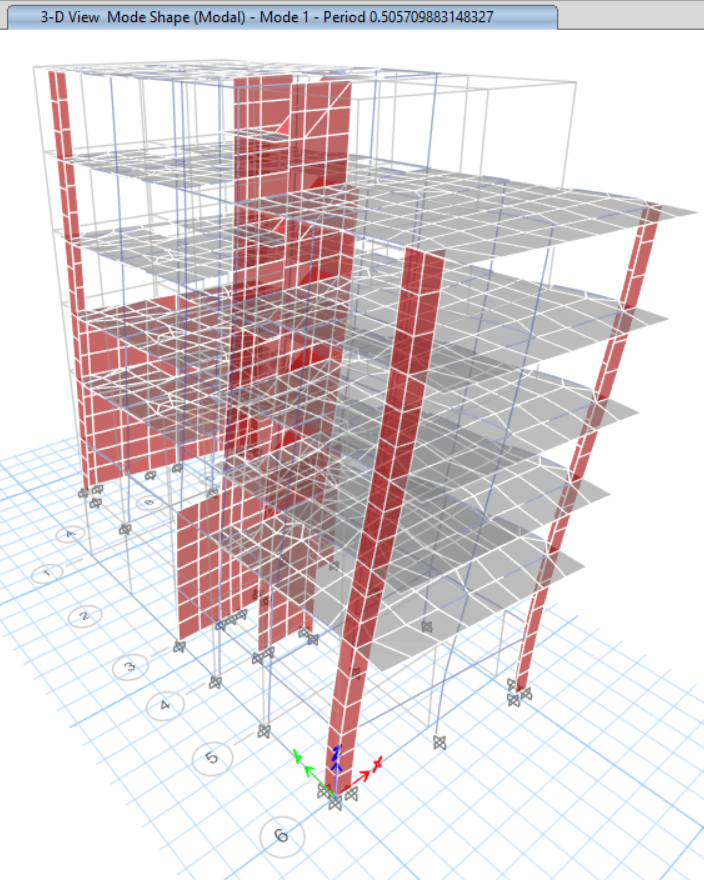
\includegraphics[height=10cm]{IMAGENES/11.PNG}
        \label{Imagen-Madrid}}
    \subfigure[2do Modo traslacional en X]{
        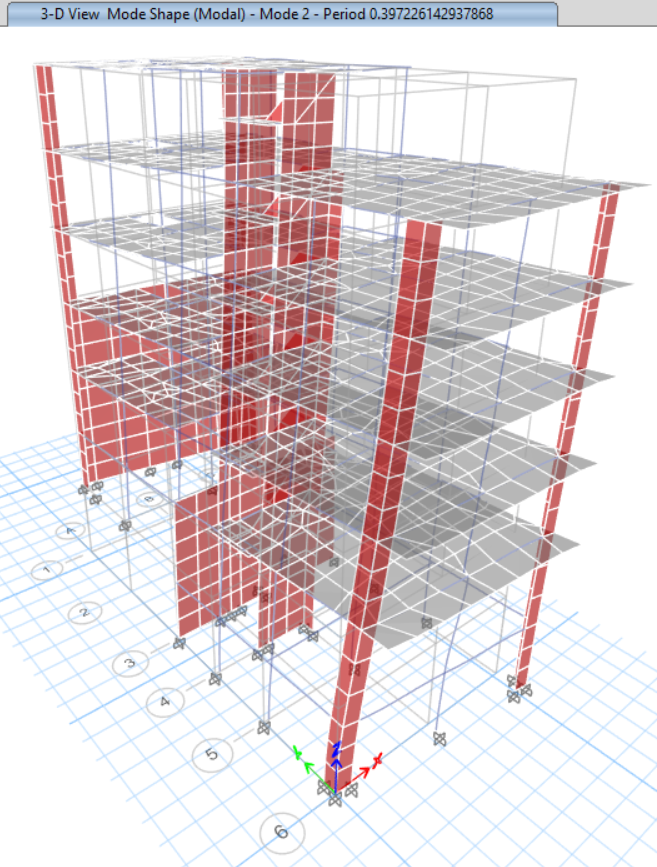
\includegraphics[height=10cm]{IMAGENES/13.PNG}
        \label{Imagen-Paris}}
    \subfigure[3er Modo torsional]{
        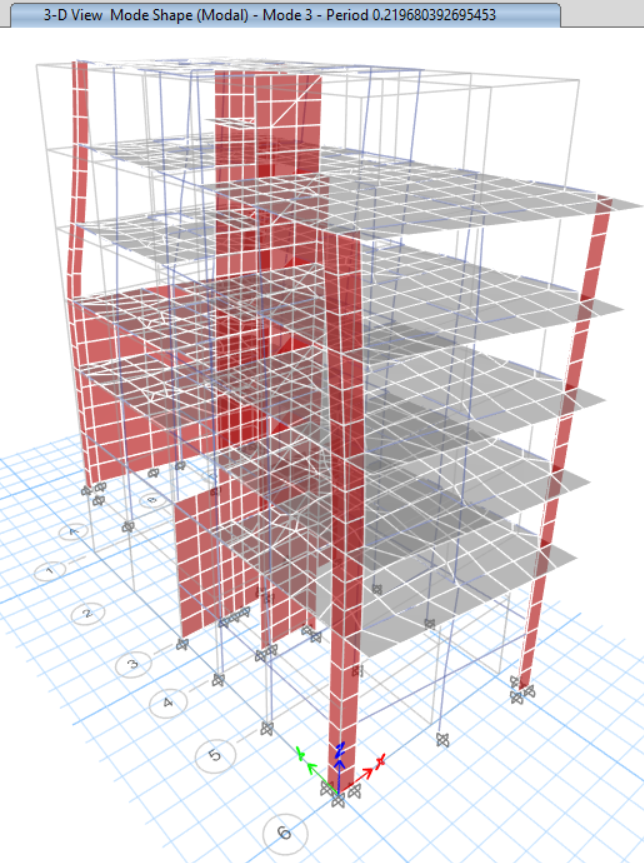
\includegraphics[height=10cm]{IMAGENES/14.PNG}
        \label{Imagen-Londres}}
    \caption{3 primeros modos de vibración}
    \label{Figura-Ciudades}
  \end{center}
\end{figure}
%\centering
%\fcolorbox{red}{yellow}{Caja de texto en amarillo con borde rojo}
%>{\centering\arraybackslash}m{2.5cm}
% Table generated by Excel2LaTeX from sheet 'Hoja5'
\newpage

\subsection{Análisis de irregularidades Art. 29 E-030}
\subsubsection{Irregularidad por discontinuidad del diafragma}
\begin{mybox2}{Tabla N°9}
\textit{La estructura se califica como irregular cuando los diafragmas 
tienen discontinuidades abruptas o variaciones importantes en 
rigidez, incluyendo aberturas mayores que 50\% del área bruta 
del diafragma.}\\
\textit{También  existe  irregularidad  cuando,  en  cualquiera de  los 
pisos y para cualquiera de las direcciones de análisis, se tiene 
alguna sección transversal del diafragma con un área neta 
resistente menor que 25\% del área de la sección transversal 
total de la misma dirección calculada con las dimensiones 
totales de la planta.}
\end{mybox2}

\begin{figure}[h!]
    \centering
    \caption{Irregularidad por discontinuidad del diafragma}
    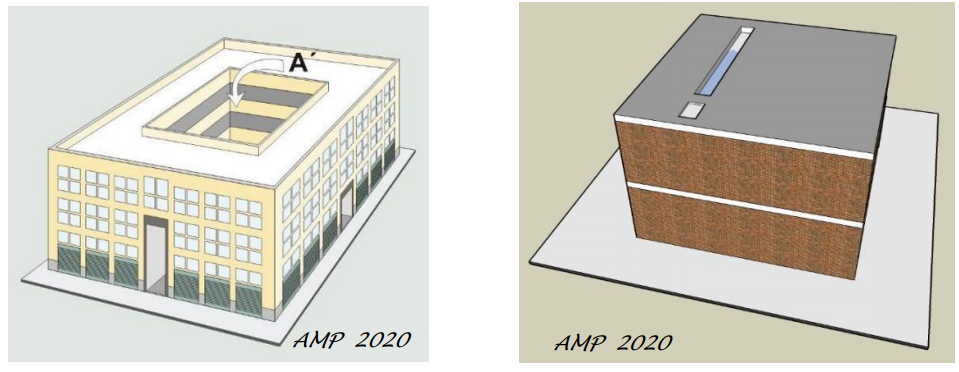
\includegraphics[scale=0.7]{IMAGENES/20.PNG}
    \caption*{\small Fuente: \it \cite{comen}}
    \label{fig:my_label}
    
\end{figure}

% Table generated by Excel2LaTeX from sheet '04) IRREG. DISCON.'
\begin{table}[h!]
  \centering
  \caption{Irregularidad por discontinuidad del diafragma (a)}
    \begin{tabular}{|ll|c|r}
\cline{1-3}    \multicolumn{2}{|l|}{Longitud del aligerado (L1)} & 7.51 & \multicolumn{1}{l}{m} \\
\cline{1-3}    \multicolumn{2}{|l|}{Espesor de losa superior del aligerado (e1)} & 0.05  & \multicolumn{1}{l}{m} \\
\cline{1-3}    \multicolumn{2}{|l|}{Area total del aligerado A1=L1.e1} & 0.38 & \multicolumn{1}{l}{m2} \\
\cline{1-3}    \multicolumn{2}{|l|}{Longitud de la losa maciza (L2)} & 2.55 & \multicolumn{1}{l}{m} \\
\cline{1-3}    \multicolumn{2}{|l|}{Espesor losa maciza (e2)} & 0.20  & \multicolumn{1}{l}{m} \\
\cline{1-3}    \multicolumn{2}{|l|}{Area de losa maciza A2=L2.e2} & 0.51 & \multicolumn{1}{l}{m2} \\
\cline{1-3}    \multicolumn{2}{|l|}{Ratio (A2/A1)} & 136.00 & \multicolumn{1}{l}{\%} \\
\cline{1-3}    \multicolumn{2}{|l|}{Limite <} & 25.00 & \multicolumn{1}{l}{\%} \\
\cline{1-3}    \multicolumn{2}{|l|}{Verificacion} & \textcolor[rgb]{ .267,  .447,  .769}{\textbf{Regular}} &  \\
\cline{1-3}    \end{tabular}%
  \label{tab:addlabel}%
\end{table}%

\begin{figure}[h!]
    \centering
    \caption{Aberturas en la planta del edificio}
    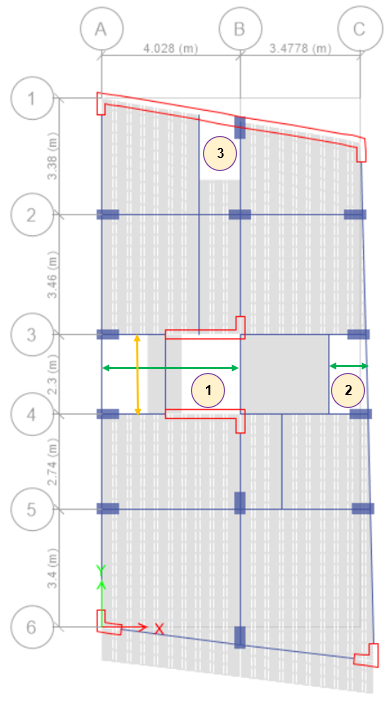
\includegraphics[scale=1]{IMAGENES/17.PNG}
    \label{fig:my_label}
\end{figure}

% Table generated by Excel2LaTeX from sheet '04) IRREG. DISCON.'
\begin{table}[h!]
  \centering
  \caption{Irregularidad por discontinuidad del diafragma (b)}
    \begin{tabular}{rr|l|c|r}
\cline{1-4}    \multicolumn{1}{|c|}{\textbf{Abertura}} & \multicolumn{1}{c|}{\textbf{Ancho (m)}} & \multicolumn{1}{c|}{\textbf{Largo (m)}} & \textbf{Area (m2)} &  \\
\cline{1-4}    \multicolumn{1}{|c|}{1} & \multicolumn{1}{c|}{4.028} & \multicolumn{1}{c|}{2.3} & 9.26  &  \\
\cline{1-4}    \multicolumn{1}{|c|}{2} & \multicolumn{1}{c|}{1.1} & \multicolumn{1}{c|}{2.3} & 2.53  &  \\
\cline{1-4}    \multicolumn{1}{|c|}{3} & \multicolumn{1}{c|}{1.2} & \multicolumn{1}{c|}{1.9} & 2.28  &  \\
\cline{1-4}          &       & Area total de aberturas & 14.07 &  \\
\cline{3-4}          & \multicolumn{1}{r}{} & \multicolumn{1}{r}{} & \multicolumn{1}{r}{} &  \\
\cline{3-4}          &       & Area total en planta  & 120.41 & \multicolumn{1}{l}{(m2)} \\
\cline{3-4}          &       & Ratio   & \textbf{11.689} & \multicolumn{1}{l}{\%} \\
\cline{3-4}          &       & Limite & \textbf{50.000} &  \\
\cline{3-4}          &       & Verificación & \textcolor[rgb]{ .267,  .447,  .769}{\textbf{Regular}} &  \\
\cline{3-4}    \end{tabular}%
  \label{tab:addlabel}%
\end{table}%

\subsubsection{Irregularidad por esquinas entrantes}

\begin{mybox2}{Tabla N°9 E-030}
\textit{La estructura se califica como irregular cuando tiene esquinas 
entrantes  cuyas  dimensiones  en  ambas  direcciones  son 
mayores que 20\% de la correspondiente dimensión total en 
planta}
\end{mybox2}

\begin{figure}[h!]
    \centering
    \caption{Irregularidad por esquinas entrantes}
    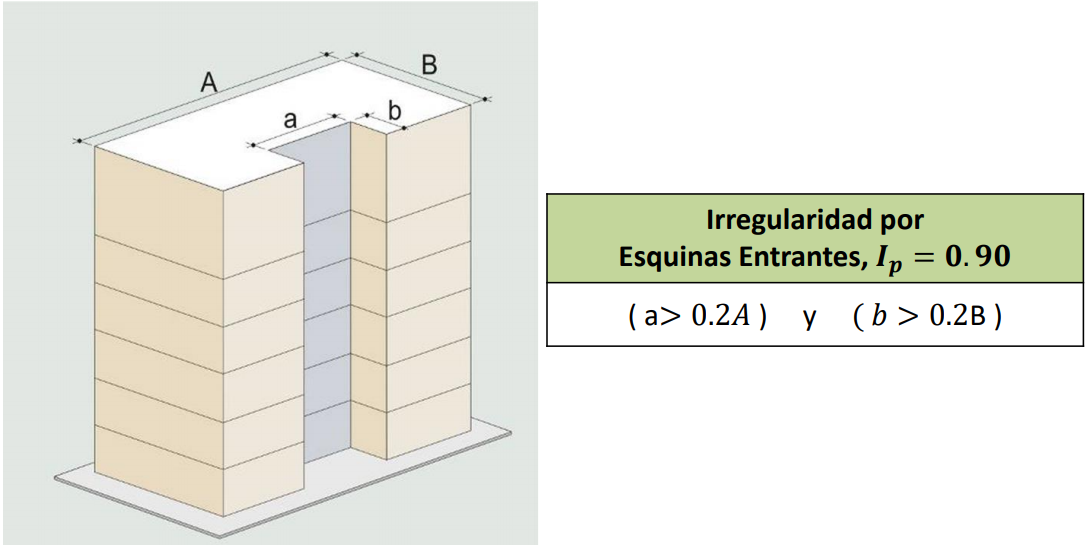
\includegraphics[scale=0.7]{IMAGENES/19.PNG}
    \caption*{\small Fuente: \it \cite{comen}}
    \label{fig:my_label}
\end{figure}

% Table generated by Excel2LaTeX from sheet '04) IRREG. DISCON.'
\begin{table}[h!]
  \centering
  \caption{Irregularidad por esquinas entrantes}
    \begin{tabular}{|ll|c|r}
\cline{1-3}    \multicolumn{2}{|l|}{Esquina entrante en X (a)} & 4.95  &  \\
\cline{1-3}    \multicolumn{2}{|l|}{Esquina entrante en Y (b)} & 2.30  &  \\
\cline{1-3}    \multicolumn{2}{|l|}{Dimension total en X (A)} & 7.51  &  \\
\cline{1-3}    \multicolumn{2}{|l|}{Dimension total en Y (B)} & 15.28 &  \\
\cline{1-3}    \multicolumn{2}{|l|}{a/A} & 66.00 & \multicolumn{1}{l}{\%} \\
\cline{1-3}    \multicolumn{2}{|l|}{b/B} & 15.05 & \multicolumn{1}{l}{\%} \\
\cline{1-3}    \multicolumn{2}{|l|}{Limite <} & 20.00 & \multicolumn{1}{l}{\%} \\
\cline{1-3}    \multicolumn{2}{|l|}{Verificación} & \textcolor[rgb]{ .267,  .447,  .769}{\textbf{Regular}} &  \\
\cline{1-3}    \end{tabular}%
  \label{tab:addlabel}%
\end{table}%


\subsection{Análisis Sísmico Dinámico Modal Espectral Art. 29 E-030}

El análisis dinámico modal espectral consiste calcular la respuesta para cada modo ingresando al espectro de pseudo-aceleraciones definido en , para posteriormente combinar los resultados según los criterios que se menciona en la norma E-030:

\subsubsection{Criterios de combinación}

\begin{mybox3}{Art. 26.3.1}
\textit{Mediante los criterios de combinación que se indican, se puede obtener la respuesta máxima elástica esperada (r) tanto para las fuerzas internas en los elementos componentes de la estructura, como para los parámetros globales 
del edificio como fuerza cortante en la base, cortantes de entrepiso, momentos 
de volteo, desplazamientos totales y relativos de entrepiso.}
\end{mybox3}

\begin{mybox3}{Art. 26.3.2}
\textit{La respuesta máxima elástica esperada (r) correspondiente al efecto conjunto 
de  los  diferentes  modos  de  vibración  empleados  (ri)  puede determinarse 
usando la combinación cuadrática completa de los valores calculados para 
cada modo.}
\end{mybox3}
\vspace{-0.8cm}
\begin{equation}
r=\sqrt{\sum \sum r_{i}\,\rho _{i}\,r_{i}}
\end{equation}
\myequations{Combinación cuadrática completa}

\begin{mybox3}{Art. 26.3.3}
\textit{Donde r representa las respuestas modales, desplazamientos o fuerzas, los coeficientes de correlación están dados por:}
\end{mybox3}

\vspace{-0.8cm}
\begin{equation}
\rho_{ij}=\frac{8\beta ^{2}\left ( 1+\lambda  \right )\lambda ^{3/2}}{\left ( 1-\lambda ^{2} \right )+4\beta ^{2}\lambda \left ( 1+\lambda  \right )^{2}}\,\,\,\,\,\,\,\,\,\,\,\lambda =\frac{\omega _{j}}{\omega _{i}}
\end{equation}
\myequations{Coeficientes de correlación}

\begin{flushleft}
Donde:\\
$\beta$: fracción del amortiguamiento crítico, que se puede suponer constante para todos los modos igual a 0,05.\\
$\omega _{j}$,$\omega _{i}$: son las frecuencias angulares de los modos i, j\\
\end{flushleft}

\subsection{Determinación de desplazamientos laterales Art. 28 E-030}
\begin{mybox3}{Art. 28.1}
\textit{Para  estructuras  regulares, los  desplazamientos  laterales  se  calculan 
multiplicando por 0,75 R los resultados obtenidos del análisis lineal y elástico con las solicitaciones sísmicas reducidas. Para estructuras irregulares, los 
desplazamientos laterales se calculan multiplicando por 0,85 R los resultados 
obtenidos del análisis lineal elástico.}
\end{mybox3}

\begin{figure}[h!]
    \centering
    \begin{tikzpicture}
    %draw[color=blue, help lines,dashed ] (0,0) grid (4.5,1.7);
    \begin{axis}
    [grid=both,
    grid style={line width=.1pt,dashed, draw=gray!10},
    major grid style={line width=.2pt,draw=gray!50},name=plot, xlabel={D (cm)},ylabel={h(m)},xmin=0,xmax=7,
    ymin=0,ymax=20,width=.6\textwidth,height=8cm,legend entries={X (R=6),Y(R=8)},legend pos=south east]%,xtick distance=.5%,ytick distance=.5]
    \addplot[OrangeRed,ultra thick,mark=o] table{./DX.txt};\label{xx}
    \addplot[MidnightBlue,ultra thick,mark=o] table{./DY.txt};\label{yy}
    \end{axis}

    \end{tikzpicture}
    \caption{Desplazamiento inelásticos}
    \label{fig:my_label}
\end{figure}

\subsection{Verificación de derivas máximas Art. 31 E-030}
% Table generated by Excel2LaTeX from sheet 'Hoja1'
\begin{table}[h!]
  \centering
  \caption{Derivas máximas}
    \begin{tabular}{|m{7cm}|c|}
    \hline
    \multicolumn{2}{|c|}{\multirow{2}[1]{*}{\textbf{LIMITES PARA LA DISTORSION DE ENTREPISO}}} \\
    \multicolumn{2}{|c|}{} \\
    \hline
    \textbf{Material predominante:} & $\Delta_{i}/h_{ei}$ \\
    \hline
    \rowcolor[rgb]{ .906,  .902,  .902} Concreto Armado & \textcolor[rgb]{ 1,  0,  0}{\textbf{0,007}} \\
    \hline
    Acero & 0,010 \\
    \hline
    Albañilería & 0,005 \\
    \hline
    Madera & 0,010 \\
    \hline
    Edificios de concreto armado con muros de ductilidad limitada & 0,005 \\
    \hline
    \end{tabular}%
    \caption*{\small Fuente: \it \cite{E-030}}
  \label{tab:addlabel}%
\end{table}%

\begin{figure}[h!]
    \centering
    \begin{tikzpicture}
    \begin{axis}
    [grid=both,
    grid style={line width=.1pt,dashed, draw=gray!10},
    major grid style={line width=.2pt,draw=gray!50},name=plot, xlabel={ $\Delta/h_{e}$},ylabel={h(m)},xmin=0,xmax=0.008,
    ymin=0,ymax=21,width=.6\textwidth,height=8cm,ytick distance=3,legend entries={X (R=6),Y(R=8)},legend pos=south east]
    \addplot[OrangeRed,ultra thick,mark=o] table{./DXX.txt};\label{xx}
    \addplot[MidnightBlue,ultra thick,mark=o] table{./DYY.txt};\label{yy}
    %\addplot[black,mark=triangle*] table{./espectro R=8.txt};\label{f}
    %\addplot[red,mark=o] table{./data/generator.txt};\label{g}
    %\addplot[blue] table{./data/simulated_total.txt};\label{s}
    %\addplot[green,dashed] table{./data/theoretical_total.txt};\label{t}
% Define two points for drawing an arrow to the "matched" point
    \node[] (C) at (axis cs: 0.007,20) {0.007};
    \node[] (B) at (axis cs: 0.007,3.5) {};
    \node[] (D) at (axis cs: 0.0035,20) {0.0035};
    \node[] (G) at (axis cs: 0.0035,0) {};
    \end{axis}
%\draw [dashed] (10,1) -- (10,11);
\draw[dashed,color=green,line width=1pt] (C)--(B);
\draw[dashed,color=orange,line width=1pt] (D)--(G);
%\node[anchor=west] (label) at (B) {matched};
    
    \end{tikzpicture}
    \caption{Derivas máximas de entrepiso}
    \label{der}
\end{figure}


\subsection{Verificación de Irregularidad torsional}
No es necesario verificar la irregularidad torsional en la dirección X dado que no se supera el 50\% de la deriva máxima permisible como se muestra en la figura \ref{der}.
\begin{figure}[h!]
    \centering
    \caption{Irregularidad torsional}
    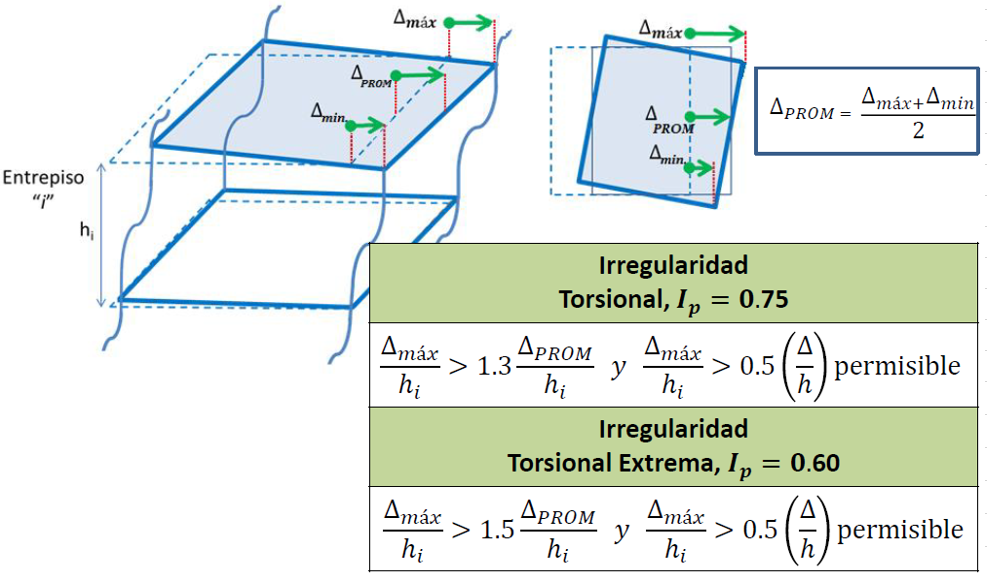
\includegraphics[scale=0.7]{IMAGENES/16.PNG}
    \caption*{\small Fuente: \it \cite{comen}}
    \label{fig:my_label}
\end{figure}

% Table generated by Excel2LaTeX from sheet 'Hoja2'
\begin{table}[h!]
  \centering
  \caption{Irregularidad torsional en la dirección Y}
    \begin{tabular}{|c|c|c|c|}
    \hline
    \multicolumn{1}{|c|}{\multirow{2}[4]{*}{\textbf{Piso}}} & \multicolumn{1}{p{5.39em}|}{\textbf{Max Drift}} & \multicolumn{1}{p{5.39em}|}{\textbf{Avg Drift}} & \multicolumn{1}{c|}{\multirow{2}[4]{*}{\textbf{Ratio}}} \\
\cline{2-3}          & \multicolumn{1}{c|}{\textbf{m}} & \multicolumn{1}{c|}{\textbf{m}} &  \\
    \hline
    6     & 0.004609 & 0.004136 & 1.114 \\
    \hline
    5     & 0.007212 & 0.006692 & 1.078 \\
    \hline
    4     & 0.010451 & 0.009752 & 1.072 \\
    \hline
    3     & 0.01278 & 0.011904 & 1.074 \\
    \hline
    2     & 0.014642 & 0.012545 & 1.167 \\
    \hline
    1     & 0.014251 & 0.012189 & 1.169 \\
    \hline
    \end{tabular}%
  \label{tab:addlabel}%
\end{table}%

El ratio no supera 1.3, por lo que el edificio en estudio no presenta irregularidad torsional.

\subsection{Verificación del sistema estructural}
Se verificara que efectivamente se tiene un sistema estructural de muros en la dirección X, en la dirección Y no se verificara dado que no existen muros estructurales. Como se muestra en la figura \ref{ver} el valor de cortante que absorben los muros es de 64 ton, y la cortante total es aproximadamente 70 ton (ver figura \ref{cor}) por lo que el porcentaje que toman los muros es mayor al 90\%.
\begin{figure}[h!]
    \centering
    \caption{Sistema estructural}
    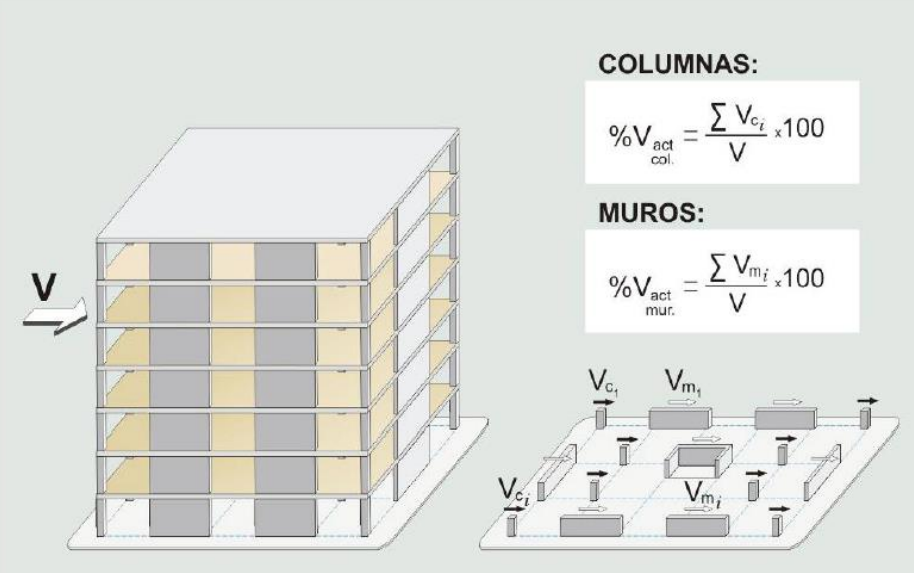
\includegraphics[scale=0.7]{IMAGENES/18.PNG}
    \caption*{\small Fuente: \it \cite{comen}}
    \label{fig:my_label}
\end{figure}
\newpage
\begin{figure}[h!]
    \centering
    \caption{Verificación del sistema estructural en X}
    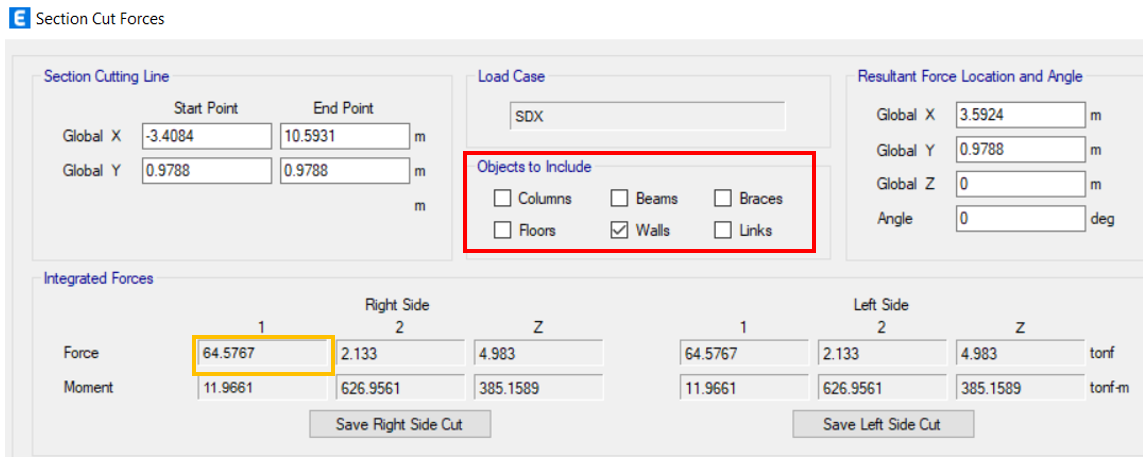
\includegraphics[scale=0.58]{IMAGENES/21.PNG}
    \label{ver}
\end{figure}

\subsection{Análisis estático o de fuerzas estáticas equivalentes Art. 25 E-030}
\subsubsection{Fuerza cortante en la base Art 25.2 E-030}

\begin{mybox3}{Art. 25.2.1}
\textit{La fuerza cortante total en la base de la estructura, correspondiente a la dirección considerada, se determina por la siguiente expresión:}
\end{mybox3}
%\vspace{-0.8cm}
\begin{equation}
V=\frac{Z\;\cdot U\cdot\;C\cdot\;S}{R}\;P\;\;\;\;\;\;\;\;\;\;\;\frac{C}{R}\geqslant 0,11
\end{equation}
\myequations{Cortante basal estática}
\noindent
Según el articulo 25.4.2 el periodo fundamental de vibración puede estimarse con la ecuación:

\begin{equation}
T=2\pi\cdot \displaystyle\sqrt{\frac{\left (\displaystyle\sum_{i=1}^{n} P_{i}\cdot d_{i}^{2}\right )}{g\cdot\left (\displaystyle\sum_{i=1}^{n}f_{i}\cdot d_{i}  \right ) }}
\end{equation}
\myequations{Periodo fundamental}
\noindent Donde:\\
$P_{i}$: es el peso sísmico en el nivel i.\\
$f_{i}$: es la fuerza lateral en el nivel i correspondiente a una distribución en altura semejante a la del primer modo en la dirección de análisis.\\
$d_{i}$: es el desplazamiento lateral del centro de masa del nivel  i en 
traslación pura (restringiendo los giros en planta) debido a las fuerzas 
$f_{i}$. Los desplazamientos se calculan suponiendo comportamiento lineal 
elástico de la estructura y, para el caso de estructuras de concreto 
armado y de albañilería, considerando las secciones sin fisurar.\\
\\
Lo anterior equivale a calcular los modos de vibrar en el modelo matemático restringiendo el grado de libertad de rotación.

\begin{figure}[h!]
    \centering
    \subfigure[X]{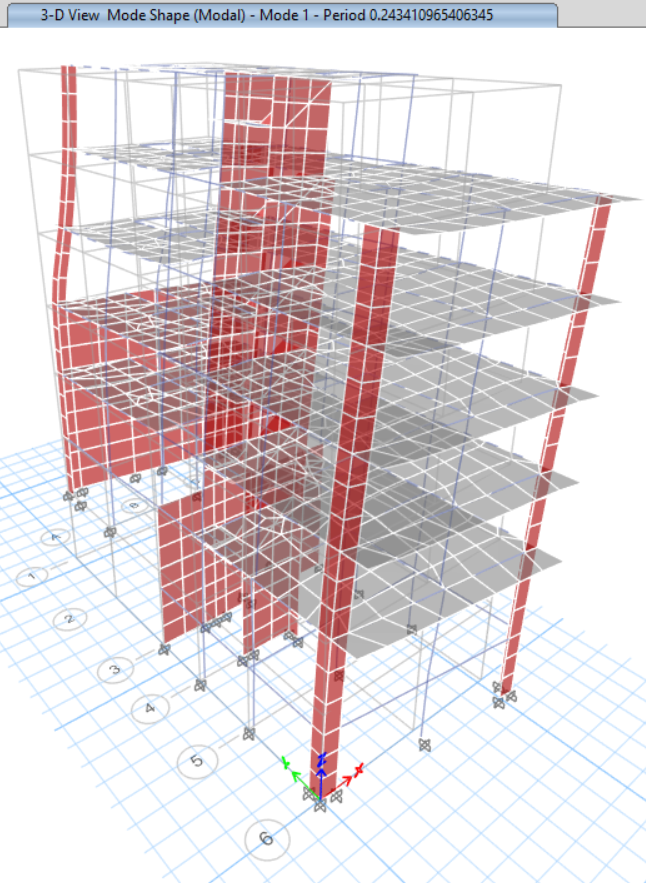
\includegraphics[height=70mm]{./TX}}\hspace{10mm}
    \subfigure[Y]{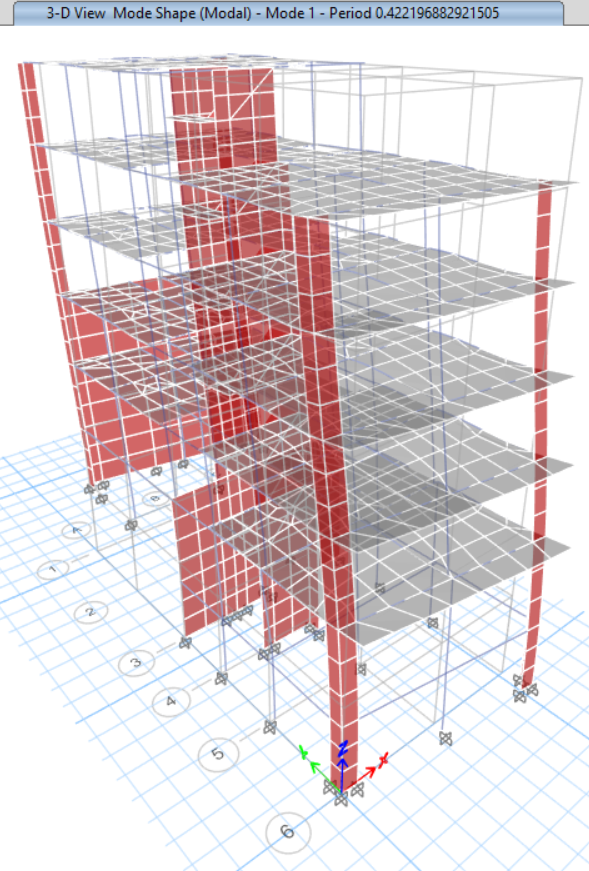
\includegraphics[height=70mm]{./TY}}
    \caption{Periodos fundamentales en traslación pura}
    \label{3}
\end{figure}
\newpage
% Table generated by Excel2LaTeX from sheet 'ASE'
\begin{table}[h!]
  \centering
  \caption{Análisis Sísmico Estático}
      {
\extrarowheight = 0ex
\renewcommand{\arraystretch}{1.2}
    \begin{tabular}{>{\arraybackslash}m{7cm}|>{\centering\arraybackslash}m{2.5cm}|>{\centering\arraybackslash}m{2cm}|>{\centering\arraybackslash}m{2cm}|}
\cline{2-4}          & \multicolumn{3}{c|}{\textit{\textbf{PARAMETROS SISMICOS}}} \\
\cline{2-4}          &       & \textbf{X} & \textbf{Y} \\
\cline{2-4}    \textit{Factor de Zona (Tabla N°1)} & \textbf{Z} & \multicolumn{2}{c|}{0.25} \\
\cline{2-4}    \textit{Factor de Uso (Tabla N°5)} & \textbf{U} & \multicolumn{2}{c|}{1.00} \\
\cline{2-4}    \textit{Periodos en traslación pura obtenidos del ETABS (Art. 25.4.2)} & \textbf{T} & 0.24  & 0.42 \\
\cline{2-4}    \textit{Factor de Amplificación (Art. 14)} & \textbf{C} & 2.50  & 2.50 \\
\cline{2-4}    \textit{Factor de Suelo (Tabla N°3)} & \textbf{S} & \multicolumn{2}{c|}{1.40} \\
\cline{2-4}    \textit{Coef. Básico de Reducción (Tabla N°7)} & \textbf{Ro} & 6.00  & 8.00 \\
\cline{2-4}    \textit{Irregularidad en altura (Tabla N°8)} & \textbf{Ia} & 1.00  & 1.00 \\
\cline{2-4}    \textit{Irregularidad en planta (Tabla N°9)} & \textbf{Ip} & 1.00  & 1.00 \\
\cline{2-4}    \textit{Coef. de Reducción (Articulo 22)} & \textbf{R} & 6.00  & 8.00 \\
\cline{2-4}    \textit{Verificación Art. 28.2.2} & \textbf{C/R$>$0.11} & 0.42  & 0.42 \\
\cline{2-4}    \textit{Carga Muerta (CM)} & \textbf{PD} & \multicolumn{2}{c|}{748.42} \\
\cline{2-4}    \textit{Carga Viva (CV)} & \textbf{PL} & \multicolumn{2}{c|}{108.84} \\
\cline{2-4}    \textit{Peso Sísmico (ETABS)} & \textbf{Ps (Ton)} & \multicolumn{2}{c|}{775.63} \\
\cline{2-4}    \textit{Coeficientes} & \textbf{ZUCS/R} & 0.15  & 0.11 \\
\cline{2-4}    \textit{Cortante Estática (Art. 28.2)} & \textbf{V (Ton)} & \cellcolor[rgb]{ 1,  .949,  .8}\textcolor[rgb]{ 1,  0,  0}{\textbf{113.11}} & \cellcolor[rgb]{ 1,  .949,  .8}\textcolor[rgb]{ 1,  0,  0}{\textbf{84.83}} \\
\cline{2-4}    Coeficiente k (Art. 28.3.2) & \textbf{k} & 1.00  & 1.00 \\
\cline{2-4}    \end{tabular}%
}
  \label{tab:addlabel}%
\end{table}%

\subsection{Fuerza cortante mínima Art. 26.4 E-030}
\begin{mybox2}{Art. 26.4.1}
\textit{Para cada una de las direcciones consideradas en el análisis, la fuerza cortante en el primer entrepiso del edificio no puede ser menor que el 80\% del valor calculado según el artículo 25 para estructuras regulares, ni menor que el 90\% para estructuras irregulares..}
\end{mybox2}

%\newmdenv[innerlinewidth=0.5pt, roundcorner=4pt,linecolor=mycolor,innerleftmargin=6pt, innerrightmargin=6pt,innertopmargin=6pt,innerbottommargin=6pt]{myboxx}

\begin{mybox2}{Art. 26.4.2 E-030}
\textit{Si fuera necesario incrementar el cortante para cumplir los mínimos señalados,  se escalan proporcionalmente todos los otros resultados obtenidos, excepto los  desplazamientos.}
\end{mybox2}
\newpage
\begin{figure}[ht!]
    \centering
    \begin{tikzpicture}
    %draw[color=blue, help lines,dashed ] (0,0) grid (4.5,1.7);
    \begin{axis}
    [grid=both,
    grid style={line width=.1pt,dashed, draw=gray!10},
    major grid style={line width=.2pt,draw=gray!50},name=plot, xlabel={V (ton)},ylabel={h(m)},xmin=0,xmax=70,
    ymin=0,ymax=20,width=.8\textwidth,height=10cm,legend entries={X (R=6),Y(R=8)},legend pos=north east]%,xtick distance=.5%,ytick distance=.5]
    \addplot[OrangeRed,ultra thick] table{./VX.txt};\label{xx}
    \addplot[MidnightBlue,ultra thick] table{./VY.txt};\label{yy}
    \end{axis}
    \end{tikzpicture}
    \caption{Cortantes de entrepiso del AME}
    \label{cor}
\end{figure}
%\vspace{-2cm}
% Table generated by Excel2LaTeX from sheet 'ESCALAM'
\begin{table}[h!]
  \centering
  \caption{Escalamiento de la cortante dinámica}
        {
\extrarowheight = 0ex
\renewcommand{\arraystretch}{1.2}
    \begin{tabular}{|l|c|>{\centering\arraybackslash}m{2cm}|>{\centering\arraybackslash}m{2cm}|}
\cline{3-4}    \multicolumn{1}{r}{} &       & \textbf{X} & \textbf{Y} \\
    \hline
    \textit{Cortante dinámica} & \textbf{V dina (Ton)} & 69.85 & 66.86 \\
    \hline
    \textit{Cortante estático} & \textbf{V est (Ton)} & 113.11 & 84.83 \\
    \hline
    \textit{Porcentaje} & \textbf{\%} & 61.75 & 78.81 \\
    \hline
    \textit{Porcentaje mínimo} & \textbf{V min \%} & 80.00 & 80.00 \\
    \hline
    \textit{Factor de escala} & \textbf{F.E.} & 1.30  & 1.02 \\
    \hline
    \textit{Cortante dinámica escalada} & \textbf{V dina esc.} & 90.49 & 67.87 \\
    \hline
    \end{tabular}%
    }
  \label{tab:addlabel}%
\end{table}%


\subsection{Separación entre edificios Art. 30 E-030}
\begin{mybox2}{Art. 30.1}
\textit{Toda estructura está separada de las estructuras vecinas, desde el nivel del terreno natural, una distancia mínima s para evitar el contacto durante un movimiento sísmico.}
\end{mybox2}

\begin{mybox2}{Art. 30.2}
\textit{Esta distancia no es menor que los 2/3 de la suma de los desplazamientos máximos de los edificios adyacentes ni menor que:}
\end{mybox2}
%\vspace{-0.8cm}
\begin{equation}
s=0.006\;h\geq0.03\;m
\end{equation}
\myequations{Separación mínima entre edificios}
\noindent Donde h es la altura medida desde el nivel del terreno natural hasta el nivel considerado para evaluar s.

\begin{mybox2}{Art. 30.2}
\textit{El edificio se retira de los límites de propiedad adyacentes a otros lotes edificables,  o  con  edificaciones,  distancias  no  menores  que  2/3  del desplazamiento máximo calculado según el artículo 28 ni menores que s/2 si la edificación existente cuenta con una junta sísmica reglamentaria.}
\end{mybox2}

\begin{figure}[h!]
    \centering
    \caption{Separación entre edificios}
    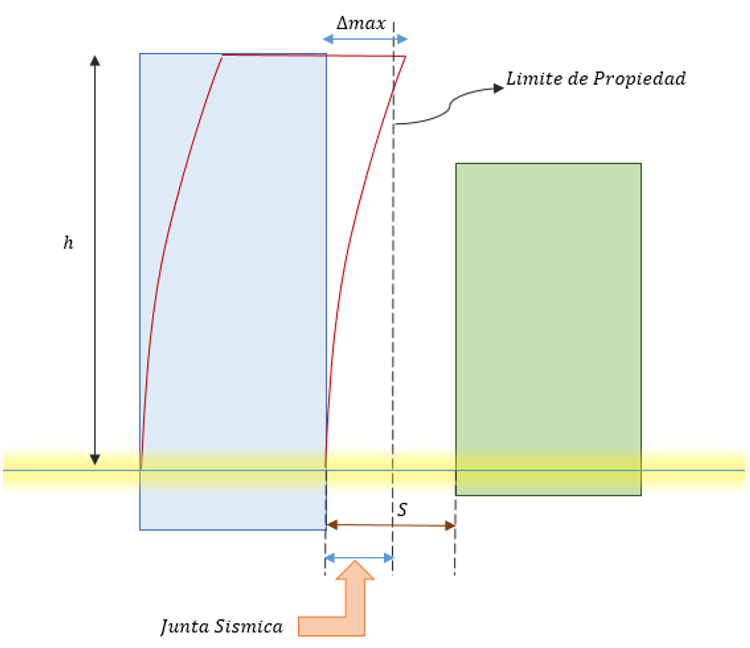
\includegraphics[scale=0.67]{IMAGENES/23.PNG}
    \label{ver}
\end{figure}
\newpage
% Table generated by Excel2LaTeX from sheet 'Hoja1'
\begin{table}[h!]
  \centering
  \caption{Calculo de la junta sísmica}
  \vspace{0.5cm}
      {
\extrarowheight = -0.3ex
\renewcommand{\arraystretch}{1.35}
    \begin{tabular}{l|c|c|l}
\cline{2-3}    \textit{Altura del edificio } & \textbf{h} & 1410.00 & cm \\
\cline{2-3}    \textit{Separación mínima entre edificios } & \textbf{s=0.006h} & 8.46  & $>$3cm \\
\cline{2-3}    \textit{Separación mínima del limite de propiedad} & \textbf{s/2} & 4.23  & cm \\
\cline{2-3}    \textit{Desplazamiento máximo en X } & \textbf{$\Delta _{x}$} & 4.81  & cm \\
\cline{2-3}    \textit{Desplazamiento máximo en Y } & \textbf{$\Delta _{y}$} & 6.07  & cm \\
\cline{2-3}    \textit{Separación del limite de propiedad X} & \textbf{2/3$\Delta _{x}$} & 3.21  & cm \\
\cline{2-3}    \textit{Separación del limite de propiedad Y} & \textbf{2/3$\Delta _{y}$} & 4.05  & cm \\
\cline{2-3}    \end{tabular}%
}
  \label{jun}%
\end{table}%

\noindent Según lo calculado en la tabla \ref{jun}  el edificio tendrá que ser separado del limite de propiedad 4.50cm como mínimo en ambas direcciones, en el caso que no exista junta reglamentaria el edificio actual se separa del edificio existente el valor de s/2 que le corresponde más el valor s/2 de la estructura vecina.

\section{Método de diseño}
Según el capítulo 9 de la norma E-060 la resistencia de diseño de todos los elementos debe ser por lo menos la resistencia requerida según:
\begin{equation}
   \phi R_{n}\geqslant R_{u} 
\end{equation}
\myequations{Requisito de resistencia según E-060}
\vspace{-1.4cm}
\section{Combinaciones de diseño}
Según el capitulo 9 de la \cite{E-060} las combinaciones de diseño serán:
    \begin{align}
        &U=1.4\;CM+1.7\;CV\\
        &U=1.25\left ( CM+CV \right )\pm CS\\
        &U=0.9\;CM+CV \pm CS         
    \end{align}
\myequations{Combinaciones de carga gravitacional}
\myequations{Combinaciones con carga sísmica 1}
\myequations{Combinaciones con carga sísmica 2}
\newpage
\noindent
Donde:\\
$CM$: Carga Muerta\\
$CV$: Carga viva\\
$CS$: Carga de sismo, según la \cite{E-030} en el artículo 21.1 el análisis se puede realizar considerando que el total de la fuerza sísmica actúa independiente en cada dirección ortogonal, por lo que se tienen 5 combinaciones independientes considerando el sismo en cada dirección.

\section{Diseño de elementos estructurales}
\subsection{Diseño de vigas}
\subsubsection{Factores de minoración}

% Table generated by Excel2LaTeX from sheet 'Hoja1'
\begin{table}[h!]
  \centering
  \caption{Factores de minoración para el diseño de vigas}
        {
\extrarowheight = 0ex
\renewcommand{\arraystretch}{1.15}
    \begin{tabular}{|>{\centering\arraybackslash}m{2.8cm}|>{\centering\arraybackslash}m{3.8cm}|>{\centering\arraybackslash}m{3.8cm}|}
    \hline
    \textbf{Articulo de E-060} & \textbf{Solicitación} & \textbf{Factor de minoración} \\
    \hline
    9.2.3.1   & Flexión & $\phi_{f}$=0.90 \\
    \hline
    9.3.2.3   & Corte y torsión & $\phi_{c}$=0.85 \\
    \hline
    \end{tabular}%
    }
  \label{tab:addlabel}%
\end{table}%
\subsubsection{Refuerzo mínimo de elementos sujetos a flexión}
\begin{mybox4}{Art. 10.5 E-060}
\textit{En cualquier sección de un elemento estructural - excepto en zapatas y losas macizas - sometidos a flexión, donde por el análisis se requiere refuerzo de acero en tracción, el área de acero que se proporcione será la necesaria para que la resistencia de diseño de la sección sea por lo menos 1.2 veces el momento de agrietamiento de la sección bruta $M_{cr}$ $\left ( \phi\;M_{n}\geq1.2\;M_{cr} \right )$.}
\end{mybox4}

\begin{flalign}
\textup{Ecu.(9.12) E-060:}\hspace{4.3cm} f_{r}=2\sqrt{f_{c}^{'}}&&
\end{flalign}
\myequations{Modulo de ruptura del concreto}
\vspace{-1.5cm}
\begin{flalign}
\textup{Ecu.(9.11) E-060:}\hspace{4.3cm} M_{cr}=\frac{f_{r}\cdot I_{g}}{Y_{t}}&&
\end{flalign}
\myequations{Momento de agrietamiento}
\noindent La norma el articulo 10.5.2 también menciona que el acero minimo en secciones rectangulares no debe ser menor que la ecuación \eqref{min}, lo cual implica que el momento resistente es aproximadamente 1.5 veces el momento de agrietamiento \cite{pasino2011}.

\begin{align}
A_{s}=\frac{0.7\sqrt{f_{c}^{'}}}{f_{y}}\cdot b_{w}\cdot d
\label{min}
\end{align}


\clearpage
\bibliography{biblio}

\end{document}

%T=A_{s}\cdot f_{y}\\
%C=0.85\cdot f_{c}^{'}\cdot a\cdot b\\
%T=C\\
%j=d-\frac{a}{2}\\
%M_{n}=T\cdot j\\